\documentclass[sigconf]{acmart}
%,letterpaper,10pt
% The preceding line is only needed to identify funding in the first footnote. If that is unneeded, please comment it out.
%\usepackage{cite}
\usepackage{amsmath,amssymb,amsfonts}
\usepackage{algorithm}
\usepackage{algorithmic}
\usepackage{multirow}
\usepackage{multicol}
\usepackage{booktabs}
%\usepackage{algorithmicx}
\usepackage{graphicx}
\usepackage{subfigure} 
\usepackage{textcomp}
\usepackage{xcolor}
%\def\BibTeX{{\rm B\kern-.05em{\sc i\kern-.025em b}\kern-.08em
    %T\kern-.1667em\lower.7ex\hbox{E}\kern-.125emX}}

\newcommand{\tabincell}[2]{\begin{tabular}{@{}#1@{}}#2\end{tabular}}

\begin{document}
	
%BIKV: Enabling a lightweight Block-conscious space reclaiming design in Key-Value Separation
\title{BIKV: Enabling a Block-conscious Space Reclaiming in Key-Value Separation}

\iffalse
\author{Huifen Chan}
\affiliation{%
	\institution{Tsinghua University}
	\streetaddress{30 Shuangqing Rd}
	\city{Haidian Qu}
	\state{Beijing Shi}
	\country{China}}
\email{cpalmer@prl.com}
\fi

\begin{abstract}
%基于LSM-tree数据结构的持久化KV存储在非顺序的负载下,LSM结构的维护会造成严重的写放大和写性能下降。KV分离的方式能缓解写放大问题同时提升写性能,然而在更新密集的负载下现有设计的管理和GC开销仍会导致写性能下降和写放大。我们基于KV分离的数据布局,提出一种就地块重用的KV存储,通过失效位置重用来减少GC开销,从而降低写放大,并提升写性能。This is realized by (i) 设计一个失效块管理器来采集、管理和重用失效位置;(ii)就地可块重用的值日志的设计。实验结果。。。
%data layout of
The Log-Structured Merge (LSM) tree that underlies many persistent key-value (KV) stores consumes significant CPU and I/O resources to maintain its data structure, resulting in high write amplification and write performance degradation. KV separation alleviates these problems by storing keys in the LSM-tree and values in a recycled log (vLog). However, the management and garbage collection (GC) overhead of current KV separation designs still takes up serious resources under GC-intensive workloads.
%decoupling key sorting and garbage collection (GC)
% in-place block-reusable KV store (IPBR-KV),设计这样的log需要在LSM-tree中进行改动,所以是实现了一个新的键值分离的KV store

We present a block-conscious in-place reused log (BILog) based on a novel block manager and implement a new KV store atop KV separation (BIKV), aiming to mitigate write amplification and improve write performance for GC-intensive workloads. The block manager gathers the invalid offsets from the discarded KV pairs in the LSM-tree, manages these offsets in blocks, and assists the GC process in the vLog. BIKV achieves hot/cold data separation by appending the valid values left in GC operations to BILog. We evaluate BIKV using microbenchmarks and compare with state-of-the-art LSM-based and KV separated KV stores via extensive experiments. Experimental results show that BIKV yields up to 3.7 X improvement in write throughput and 44\% degradation in write amplification compared to the current KV separation design. When it accumulates large volumes of invalid offsets under update-intensive workloads, BIKV almost eliminates the write amplification and GC overhead in BILog.
%(i) extracting the offsets of stale values in BILog from the discarded KV items in the LSM-tree, (ii) building a block manager to collect and manage these offsets, and (iii) realizing a lightweight GC based on the state of blocks. 
%designs a flushing data location selector based on the invalid block reuse modes 
%It yields up to 70% improvement in write throughput and reduces write amplification by a factor of up to 2x compared to the current KV separation design.
%achieves 4.6× throughput and 53.4\% less write traffic compared to the current KV separation design under update-intensive workloads.
%yields up to 193% improvement in throughput. It reduces write amplification by a factor of up to 4x, and decreases the amount of I/O by an order of magnitude.
%designing an invalid block reuse policy, and (iii) implementing an in-place block-reusable recycled log.

\end{abstract}

\keywords{Key-Value Store, Key-Value Separation, Data Management}

\maketitle

\section{Introduction}
%首先是LSM-based结构的KV store的广泛使用及其存在的问题:compaction操作造成的写放大,以及对前台写性能的影响。
Persistent key-value (KV) stores play a crucial role in modern data-intensive applications, such as messaging \cite{HH,HBase}, e-commerce \cite{Dynamo}, search indexing \cite{LevelDB, Bigtable} and advertising \cite{RocksDB,PNUTS}. Various modern large-scale KV stores are built on Log-Structured Merge tree (LSM-tree) \cite{LSMtree} to benefit from sequential access patterns for writes, such as LevelDB \cite{LevelDB}, RocksDB \cite{RocksDB}, Bigtable \cite{Bigtable}, HBase \cite{HBase}, Cassandra \cite{Cassandra} and bLSM \cite{bLSM}, etc.
%Log-structured merge tree (LSM-tree) \cite{LSMtree} is a disk-based index structure, performing out-of-place updates to achieve sequential writes of entries, to deliver high write performance. To enable efficient lookups, the LSM-tree maintains entries in sorted order. Thus as it receives more writes, it needs to continuously read, sort, and write the entries in the background, this process is called the rolling merge. 
%The LSM-tree is employed in a wide range of persistent key-value (KV) stores, such as LevelDB \cite{LevelDB}, RocksDB \cite{RocksDB}, Cassandra \cite{Cassandra}, and bLSM \cite{bLSM}. 
%In most LSM structured KV stores (LSMs), the rolling merge which is indispensable to maintain the data structure, is called compaction \cite{LevelDB, HyperLevelDB, RocksDB}. For write-intensive workloads, as the LSM-tree grows in size, it will trigger frequent compaction operations, resulting in large amounts of write IO. 

As the LSM-tree grows in size, the LSM-tree necessitates the compaction operation to maintain the data organization and provide efficient write and read performance, which results in large amounts of write IO under write-intensive workloads \cite{LevelDB, HyperLevelDB, RocksDB}. The ratio of total write IO performed by the store to the actual writes is called write amplification \cite{LevelDB, PebblesDB}. Such write amplification can reach a factor of at least 17 X \cite{Wisckey,PebblesDB}, which is detrimental to the endurance of SSD \cite{SSD, Wisckey, HashKV}. Besides, even though the compaction occurs outside the critical path of user-oriented operations, it takes up significant CPU and I/O resources, resulting in that the writing progress at the front end is often stalled or blocked, thus disturbs the write performance of the LSM structured KV stores \cite{TRIAD, PebblesDB}. 
%The LSM-tree also incurs high read amplification (i.e., a lookup operation always reads more data than its demand). Such read amplification can reach a factor of over 300× when reading the KV pairs at lower levels which incurs many disk accesses, thus leads to low read performance \cite{Wisckey}.

Many research efforts focus on optimizing the compaction strategy of the LSM structured KV stores to improve write performance \cite{HyperLevelDB,bLSM,PCP,cLSM,CM} and decrease write amplification \cite{LSMtrie,skiptree,LWCtree,TRIAD}. While some other approaches separate keys from values to fundamentally reduce the number of compaction, such as Wisckey \cite{Wisckey} and HashKV \cite{HashKV}. The KV separated stores consist of a key store (e.g., the LSM-tree) and a value store (i.e., a recycled log). KV separation is present to be highly SSD optimized to significantly reduce write amplification while preserving the efficient writes, point lookup, and range queries by leveraging both the sequential and random performance characteristics of the SSD device.

%摘
% The success of LSM-based technology is tied closely to its usage in classic hard-disk drives (HDDs), in which performing additional sequential reads and writes to I/Os are over 100× slower than sequential ones.
%Write amplification is the ratio of total write IO performed by the store to the total user data. High write amplification increases the load on storage devices such as SSDs, which have limited write cycles before the bit error rate becomes unacceptable [3, 26, 39].

%面向SSD的适用性问题,提出了wisckey,用一种KV分离的方法,用LSM-based结构的KV store作为key store part,将value以append-only的形式存储在循环value log(vlog)中,通过GC操作清理失效KV,获得可用空间。实验结果证明对于random load的负载其在写放大和写性能方面都优于leveldb。然而存在GC的wisckey性能比无GC(vlog空间足够)的性能差[Wisckey],尤其是面向更新密集的应用时,产生大量的GC操作,不仅会造成写性能降低,还会造成严重的写放大[Hashkv]. 为了优化面向更新密集型复杂,Wisckey产生的大量GC带来的严重写放大和较大的GC开销,hashkv通过分区,设置多个segment ,使得同一个key会落到同一个segment,GC时不需要查询LSM-tree来判断有效性,然而hashkv中segment管理复杂,使得他在并行度不够的情况下写性能较差,而且仍然存在一定的写放大。
When the values in the value store accumulates to a threshold size, the KV separated stores start to trigger garbage collection (GC) to discard the stale values and reclaim space. In Wisckey, large numbers of GC significantly decreases the write performance because of the substantial GC overhead \cite{Wisckey} and arouses large amounts of data rewrites in the value store under update-intensive workloads \cite{HashKV}. To mitigate the GC overhead under update-intensive workloads, HashKV uses hash-based data grouping to deterministically map values to storage space and make GC efficient which leads to better write performance than Wisckey under frequent GC. However, HashKV has lower write performance than Wisckey before both of them start to trigger GC because of the complex management of data groups.
%However, compared to Wisckey, HashKV has lower write performance until both of them start to trigger GC. The reasons are the complex management of data groups in HashKV harms write throughput, while the optimized GC process based on data groups reduces the GC overhead.

%***************动机需要再写清楚一些,摘自hashkv,需要根据自己的特色提出问题
%This can incur a large amount of unnecessary data relocation (e.g., when the least recently written KV pairs remain valid). Second, the GC operation needs to query the LSM-tree to check the validity of each KV pair. These queries have high latencies, especially when the LSM-tree becomes sizable under large workloads. 

%提出一种支持就地更新的键值分离的键值存储系统,利用compaction中drop的KV管理vlog的失效KV状态从而实现就地更新,通过这种操作降低GC频繁和GC开销,从而减少写放大。
In this paper, we present a block-conscious in-place reused log (BILog) based on a novel block manager as the value store in KV separation and implement a new KV store atop Wisckey (BIKV), aiming to improve the write amplification and write performance under GC-intensive workloads (i.e., write-intensive workloads result in frequent GC). BIKV strikes at the root of GC overhead by utilizing the discarded KV pairs in the key store whose value includes the offset of a stale value in the value store. The block manager consists of a large number of blocks that deterministically map to fixed-size segments in the value store. Each block involves several continuous offsets which are the starting positions of values in the value store. The block manager extracts the offsets from the discarded KV pairs in the key store called invalid offset, manages these offsets in blocks and assists reclaiming the storage space in the value store. Based on the block manager, we implement BILog and provide a lightweight GC strategy in BIKV. When it starts to trigger GC, BIKV reclaims space by recycling the candidate blocks, and subsequently performs in-place updates to the segments these blocks map to when flushing the new data. BIKV realizes the hot/cold data separation by appending the valid data left in a GC operation to the tail of BILog.

%the memory cost for the block manager and
The design of BIKV brings about an additional crash consistency issue: the recovery of the metadata (i.e., the states of offsets in blocks) in the block manager. We record the metadata to recover the KV store. Without recovering the block manager, BIKV degenerates to Wisckey at initially recovered. BIKV is suitable for fixed-size KV pairs, while for variable-size KV pairs it would result in space waste in each block and complex block management. In this paper, we focus on observing the write performance and write amplification of BIKV under GC-intensive workloads; thus, we only experiment with the fixed-size KV pairs in the evaluation.
% bring about the fundamental problem of write amplification and decrease write performance

% 就地更新使得系统较适用于固定大小的KV,非固定大小的KV管理更复杂,且会存在一定的空间浪费,本文只讨论固定大小KV;由于逐个就地更新对SSD不友好,因此设计批量就地更新,最小公倍数,最后构建一个块可重用的键值分离的键值存储系统;对于一致性问题,锁;可恢复性,日志
%The nature of in-place updates makes NG-KV be constrained to two factors: (1) the size of KV pairs which should be fixed or consistent with some distributions, such as the lengths of most KV pairs are close (i.e., in a threshold range) which would result in a little space waste; (2) the storage device which should be HDD or byte-addressable NVM. Thus, we evaluate NG-KV with fixed size of KV pairs on the hybrid store devices (i.e., SSD and HDD). On the other hand, the GC-free design brings about the crash consistency issue. Thus, we propose two design extensions to guarantee recoverability: (1) batch in-place updates, the design pattern is much like Memtable and immutable Memtable; (2) in-place updates log, which is used to recover the state of vLog. 

%实现以及效果
We implement BIKV upon \textit{vLog} implementation in the prototype of HashKV \cite{HashKV}, and evaluate BIKV with the testbed in HashKV. We extensively compare BIKV against state-of-the-art KV separated (i.e., Wisckey and HashKV) and LSM structured KV stores (i.e., LevelDB, HyperLevelDB and PebblesDB). The experimental results show that BIKV achieves 3.7 X throughput and 44\% less write traffic compared to WiscKey and HashKV under GC-intensive workloads. BIKV almost eliminates data rewrites to the value store when it tiggers GC with abundant entirely invalid blocks, drastically reducing write amplification and improving write throughput.
%generally achieves higher throughput and significantly less write traffic compared to modern KV stores, such as LevelDB and RocksDB, in various cases.  

%In summary, this paper makes the following contributions: (1) the design and implementation of a novel GC-free key-value separated KV store, NG-KV, which utilizes the invalid KV pairs that generated in compaction processes of the LSM-structured key store part, to realize in-place updates (\ref{sec3}); (2) an evaluation of NG-KV in comparison to the state-of-art KV separated stores and LSM-based stores, in which the experimental results demonstrate that NG-KV dominates those KV stores which are run on SSD, achieving low write amplification and high write throughput (\ref{sec4}).
%测试读性能,对于YCSB的benchmark应该读性能也会提升

\textbf{Roadmap}. The rest of the paper is organized as follows. Section 2 describes the motivation. Section 3 presents the design and implementation of BIKV. Section 4 analyzes the performance of BIKV. Section 5 discusses related work. Section 6 concludes this paper.

\section{Motivation}
%19-10.8 是不是应该简单介绍LSM结构,具体介绍Wisckey和HashKV?
In this section, we explain the problems of write amplification and write performance degradation in LSM structured stores and KV separated stores caused by compaction and garbage collection, respectively.

%从LevelDB去讲写放大和写性能的问题
\paragraph{LevelDB} LevelDB \cite{LevelDB} is a representative LSM structured stores and also used as the key store in KV separated stores. Fig.~\ref{fig::lsm_wisckey} (a) illustrates the data organization in LevelDB, which consists of two components: a memory component and a disk component. 

The memory component is used to batch up small random writes, keep them in sorted order and form sequential writes, hence maintains high write performance and efficient queries. It has two parts residing in main memory, called Memtable and immutable Memtable, in which KV pairs are organized in a skiplist \cite{skiplist}. The size of Memtable is usually ranging from a few megabytes (MBs) to tens of MBs. The disk component typically includes four parts: a commit log, an operation log, metadata, and data. The commit log is a write-ahead log, used to avoid data loss. The operation log is used to check the execution state of the KV store. The metadata file is used to recover the KV store. Data (i.e., KV pairs) is organized into multiple levels, such as $k$ levels, denoted by $L_0$, $L_1$,$\ldots$, $L_{k-1}$ (e.g., 7 levels default in LevelDB). The capacity of each level is configured to be a multiple of that of its upper level (e.g., 10 X default in LevelDB). Each level contains many data files which store KV pairs in sorted order, called Sorted String Table (SST). The size of SST is also ranging from a few MBs to tens of MBs.

As shown in Fig.~\ref{fig::lsm_wisckey} (a), when writing a KV pair, first insert it into the commit log (a.1), and then insert it into Memtable (a.2). When the volume of data in Memtable accumulates to its target size, Memtable turns into immutable Memtable (a.3), and then a new Memtable is created. The immutable Memtable is subsequently flushed to the disk component (a.4). If the number of SST in $L_0$ accumulates to the threshold, it triggers a compaction operation (a.5). With the increasing of data volume, it triggers frequent compaction from top level to bottom. The process of compaction is 1) selecting one or more SSTs from $L_i$ (where 0$\le$$i$$\le$$k-1$)  and several SSTs in overlapping key range from $L_{i+1}$; 2) merging and sorting the KV pairs in these SSTs to discard the stale KV pairs and 3) rewriting the sorted KV pairs into new SSTs to $L_{i+1}$. Even though it occurs in the background, compaction still consumes significant resources, thus disturbs the write performance of LSM structured stores.

When reading a KV pair, it keeps looking for the key until finding it, and the query sequence is 1) Memtable; 2) Immutable Memtable; 3) several SSTs in overlapping key range from $L_0$; 4) at most one SST in overlapping key range from the rest of levels. With the increasing size of the KV store, the read performance becomes worse.

%such as $L_i$ (where 0$\le$$i$$\le$$k-1$) exceeds its target size, it triggers a compaction operation (a.4). The process of compaction is selecting one or more SSTs from $L_i$ and several SSTs in overlapping key range from $L_{i+1}$, merging and sorting these KV pairs, discarding stale KV pairs and rewriting valid KV pairs into new SSTs to $L_{i+1}$. 

%Compaction is indispensable to maintain the LSM-tree structure. Unfortunately, even though it occurs in the background, it still consumes significant resources, including a set of reads, writes, and file operations thus disturb the write performance of LSMs. The overhead of each compaction is so large that the LSM-based KV stores use multiple levels to amortize the cost of compaction for write-intensive workloads \cite{TRIAD}. However, it leads to severe write amplification.

%the write and read are user-oriented operations, while flushing and compaction are background operations. Because of the flushing operation, the key range of SSTs at $L_0$ is always overlapped between each other under random write workloads, while SSTs at the remaining levels have disjoint key ranges due to the compaction operation. Compaction and flushing are indispensable to maintain the LSM-tree structure. However, even though they occur outside the critical path of user-oriented operations, they still take up a significant amount of the available resources, resulting that write operations are often stalled or blocked.

%To provide efficient read and range query performance, the compaction operation is necessary \cite{PebblesDB}. The overhead of each compaction is large, including a set of reads, writes and file operations. Thus, the LSM-based KV stores use multiple levels to amortize the cost of compactions for write-intensive workloads \cite{TRIAD}, and it leads to severe write amplification.

% Leveldb, Wisckey图
\begin{figure}[!t]
	\setlength{\abovecaptionskip}{0.cm}	
	\setlength{\belowcaptionskip}{-0.cm}
	\centerline{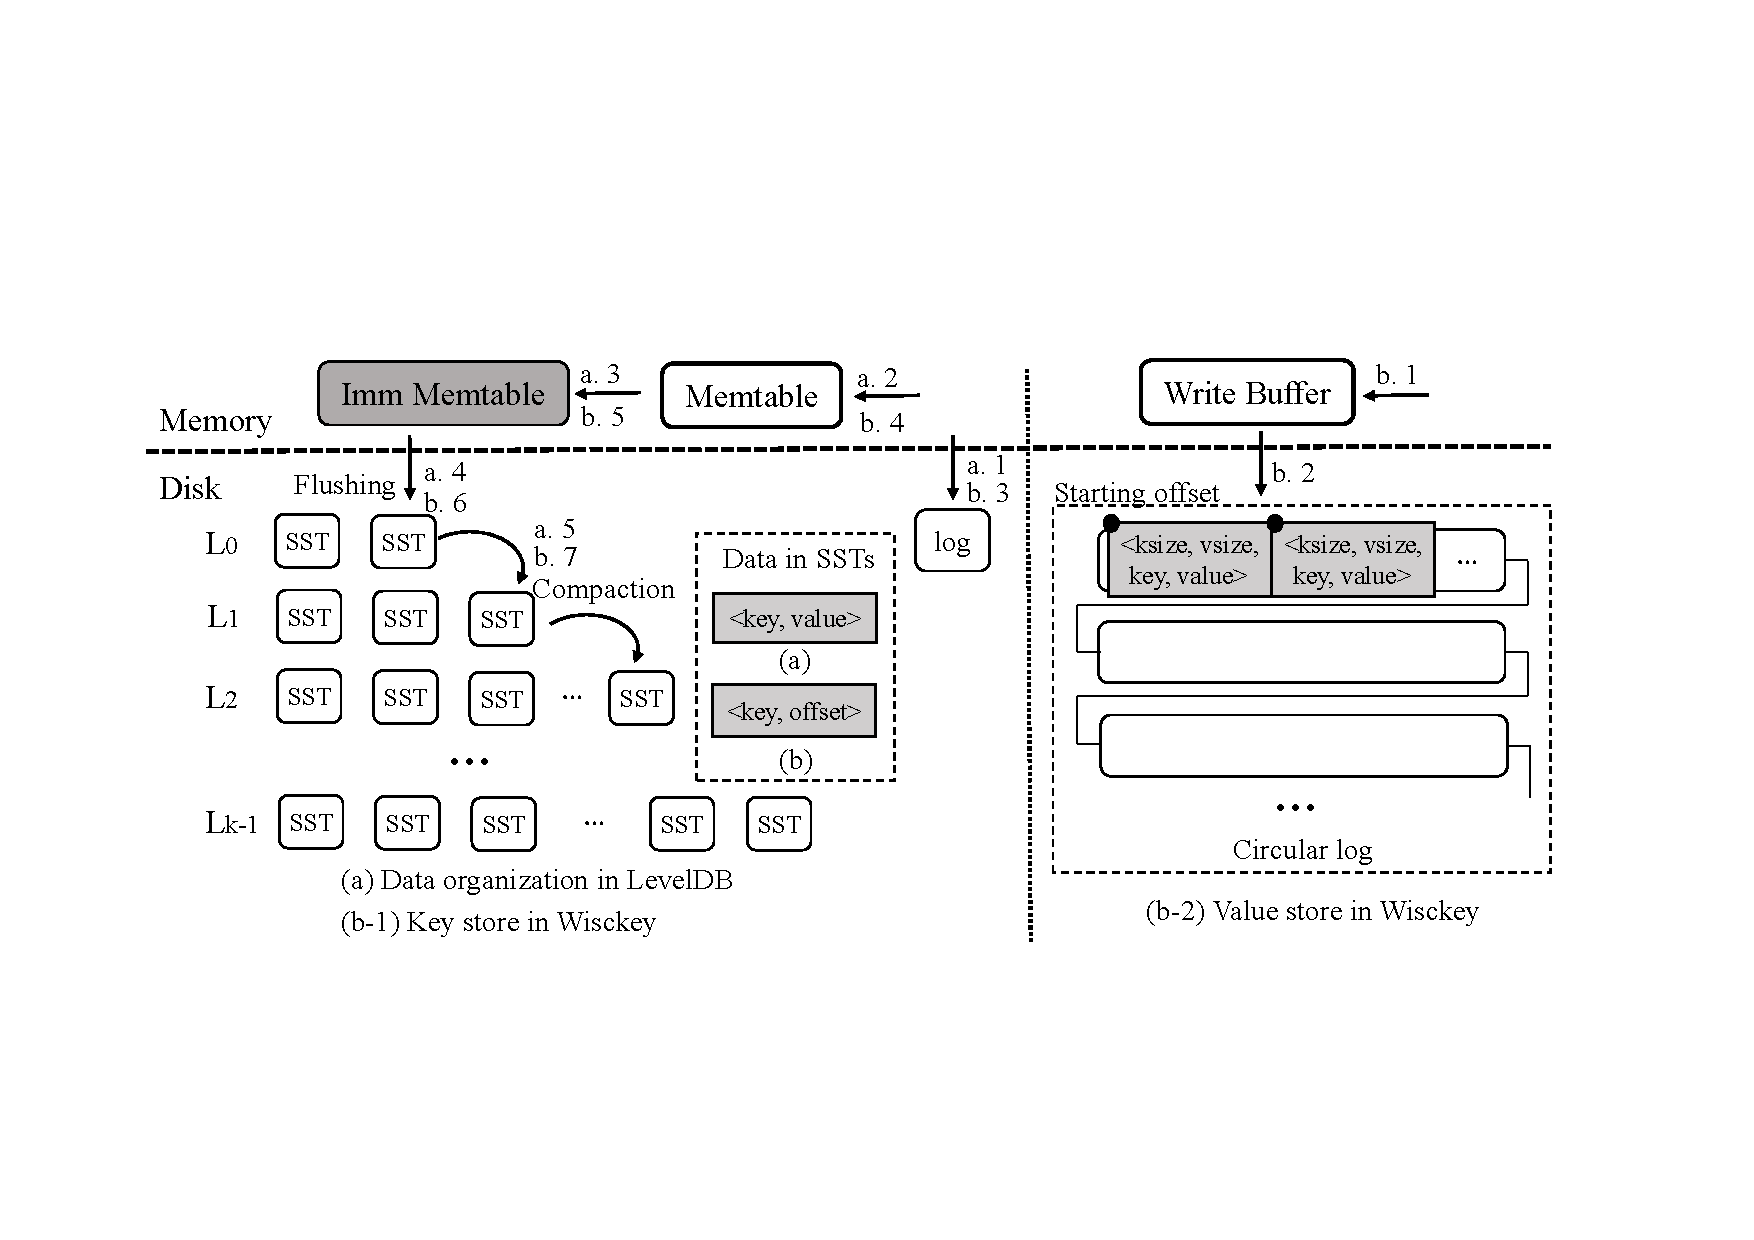
\includegraphics[width=80mm]{lsm_wisckey.pdf}}
	\caption{LevelDB and Wisckey architecture.}
	\label{fig::lsm_wisckey}
\end{figure}

%Wisckey的初衷是优化SSD上LSM结构的KVstore的写放大问题,然而由于GC开销大,若是产生大量的GC会造成Wisckey严重写放大并影响写性能
%对于操作,读操作在LSM中找到offset,在LOG里面读出KV;写操作先写vlog,再将元数据更新到LSM;删除操作,直接写到LSM
% operations to discard the invalid KV pairs and release the space
\paragraph{Wisckey} Wisckey is an SSD-conscious persistent KV store derived from LevelDB, which separates keys from values to significantly mitigate the write amplification so as to improve the endurance of SSD. The separated keys are used as indexes of the values. Fig.~\ref{fig::lsm_wisckey} (b) illustrates the data organization in Wisckey, which consists of a key store and a value store. The key store is an LSM structured store called the LSM-tree, e.g., LevelDB which is briefly introduced above.

The value store also includes a memory component and a disk component. The memory component is a write buffer, used to avoid the noticeable overhead caused by a large number of small writes to a file system, especially on a fast storage device for a write-intensive workload \cite{Arrakis, Wisckey}. The disk component is an append-only circular log called vLog. As shown in Fig.~\ref{fig::lsm_wisckey} (b), when writing a KV pair, first append it to the write buffer (b.1). When the buffer size exceeds its target size, it is flushed to vLog in the form of tuple \textless key size, value size, key, value\textgreater{} (b.2). Then bulk insert the keys along with the values’ info \textless vLog-offset, value-size\textgreater{} into the LSM-tree (b.3). The subsequent operations are as described above.

When executing a point lookup, it first queries the key in the LSM-tree. The process is described above. If the key exists, it gets the value and extracts the vLog-offset from the value. Secondly, read the KV pair at the offset in the vLog.

When the data volume in the vLog accumulates to a threshold size, it starts to trigger garbage collection (GC) to free space in the vLog and keep valid values (not overwritten or deleted) in a contiguous range of the vLog. Wisckey set two pointers to recognize the valid range of vLog: (1) the \textit{head}, the end point to append new values; (2) the \textit{tail}, the start point of GC. The process of GC in WiscKey is 1) reading a chunk of key-value pairs (e.g., 64 MB) from the tail of the vLog, 2) finding which of those values are valid by querying the LSM-tree, 3) appending valid values to the head of the vLog, and 4) freeing the space occupied previously by the chunk and updates the tail accordingly. Thus, GC results in data rewrites and also costs significant resources, both affect write performance.  In particular, real-world KV storage often exhibits strong locality \cite{Workload}, in which a small portion of KV pairs are frequently updated (i.e., hot data), while the remaining KV pairs receive only few or even no updates (i.e., cold data). Sequential GC order in vLog inevitably relocates cold data many times and increases GC overhead \cite{HashKV}.

\paragraph{HashKV} HashKV \cite{HashKV} is a KV separated store, aiming to mitigate the GC overhead under update-intensive workloads. The value store consists of vLog and reserved space. HashKV partitions vLog into fixed-size segments called main segment, and maps values into partitions in the vLog by hashing the associated keys. HashKV also partitions reserved space into segments called log segment, and allows a partition to grow dynamically beyond its size limit by allocating the KV pairs to reserved space. Thus, each partition includes one main segment and several log segments, called segment group. HashKV separates the storage of hot and cold KV pairs with a cold data block, to apply GC to hot KV pairs only and avoid re-copying cold KV pairs. 

In HashKV, it starts to trigger GC when the free log segments in the reserved space are running out. The process of GC is 1) selecting a candidate segment group, 2) identifying all valid KV pairs in the group, 3) writing back the valid KV pairs to the main segment, or additional log segments if needed, in a log-structured manner, 4) releasing any unused log segments which can be later used by other segment groups and 5) updating the latest value locations in the LSM-tree. HashKV sequentially scans the KV pairs in the segment group to identify the valid KV pairs (i.e., the KV pairs of the latest version) without querying the LSM-tree, thus significantly mitigate the GC overhead. Based on hotness awareness, HashKV mitigates write amplification and improves write performance.

%实验结果(leveldb, wisckey),从没有这些操作和频繁的操作所产生的写吞吐量和整体写入量,说明写放大和写性能问题
% and HashKV \cite{HashKV},HashKV builds atop KV separation and uses hash-based data grouping to map from values to storage space, combining with several design extensions to achieve both updates and GC efficient under update-intensive workloads. 
\paragraph{Experiments for Compaction and GC} We do a set of experiments on LevelDB (Version 1.20), Wisckey and HashKV, to demonstrate the impact of compaction and GC on write performance and write amplification. In the experiments, the KV size is of 1 KB. We use single-threaded micro-benchmarks to evaluate the performance of LevelDB on 40 millions (M) writes in sequential write (\textbf{SW}) and random write (\textbf{RW}) manner. We use the testbed in HashKV \cite{HashKV} to evaluate Wisckey and HashKV on 40 M random writes (\textbf{Load}) and 12 M updates (\textbf{Update}), resulting in about (39 GB, 1.9 GB) and (12 GB, 0.78 GB) writes to vLog and the LSM-tree, respectively. 
%For LevelDB, the Memtable size is of 32 MB and the SST size is of 16 MB.  For Wisckey, the capacity of vLog is of 42 GB and the size of data chunk in each GC is of 64 MB.  

We run the experiments with these parameters as follows:
\begin{itemize}
	\item LevelDB: Memtable size (32 MB), SST size (16 MB); 
	\item Wisckey: vLog capacity (42 GB), GC unit (64 MB); 
	\item HashKV: vLog capacity (40 GB), reserved space (2 GB), GC unit (segment group).
\end{itemize}

%The experimental results are shown in Table \ref{table:mo}. \textbf{WT}, \textbf{TW}, \textbf{C} and \textbf{GC} stand for write throughput, total write (represented in form of "vLog + LSM-tree" for KV separation stores), the number of compaction and the amount of GC, respectively.

The experimental results are shown in Table \ref{table:mo}. \textbf{WT}, \textbf{TW}, \textbf{C} and \textbf{GC} stand for write throughput, total write, the number of compaction and the number of GC, respectively. For KV separated stores, the total write is represented as the writes in (vLog, LSM-tree). Note that, Wisckey and HashKV start to trigger GC in update phase.
% 要改LevelDB RW............
\begin{table}[!t]
	\setlength{\abovecaptionskip}{0.cm}	
	\setlength{\belowcaptionskip}{-0.cm}
	\centering
	\caption{The negative impact of compaction and GC on write performance and write amplification. }
	\label{table:mo}
	\scalebox{0.8}{	
	\begin{tabular}{ccccccc}
			\toprule
			\multirow{2}{*}{\textbf{Metrics}} & \multicolumn{2}{c}{\textbf{LevelDB}} & \multicolumn{2}{c}{\textbf{Wisckey}} & \multicolumn{2}{c}{\textbf{HashKV}} \\
			\cmidrule(lr){2-3} \cmidrule(lr){4-5} \cmidrule(lr){6-7}
			& SW &  RW &  Load & Update & Load & Update \\
			\midrule
			WT (MB/s) & 77.1 & 7.0 &  103.4 & 8.6 & 63.9 & 11.9 \\
			TW (GB) & 39 & 475 & (39, 17) &  (29, 78) & (39, 26) & (64, 43) \\
			C & - & 6466 & 1563 & 4536 & 2109 & 4329 \\
			GC & - & - & - & 103 & - & 879 \\
			\bottomrule
	\end{tabular}
	}
\end{table}

%leads to an order of magnitude write amplification problem
%根据结果分析compaction对LSM-based KV store的性能影响,更新密集型应用对Wisckey的影响,hashkv,wisckey的写性能和总体写入量
As shown in Table \ref{table:mo}, LevelDB provides excellent write performance for sequential writes. However, for random writes which generate large amounts of compaction, the write throughput (WT) is significantly decreased, and the ratio of write amplification (WA) is more than 12X. 

For KV separated stores, in load phase, Wisckey has the best WT for random writes and no data rewrites in the vLog, but there is more than 8 X WA in the LSM-tree because of compaction; WT of HashKV is worse because of the complex segment management, WA in the LSM-tree is more than 13 X, and the reason of the difference with that in Wisckey is that the sequence of keys inserted to the LSM-tree is different.

When it starts to trigger GC in update phase, the number of GC in HashKV is much more than that in Wisckey, resulting in worse WA of HashKV in the vLog. WT of them both severely decreases, while WT of HashKV is better than that of Wisckey benefiting from the optimized GC strategy. Both of them generate severe WA in the LSM-tree because of large numbers of compaction. 
%The difference on total write between them may result from the various insert sequence of keys. 

%and more than 2X write amplification in vLog. In the LSM-tree, it generates large amounts of compaction and more than 100X write amplification. 

%HashKV has lower write performance than Wisckey in the load phase because of its complex segment management. In the update phase, HashKV arouses more GC operations, resulting in more than 5X write amplification in vLog, but the optimized GC makes the write performance more efficient. Although it generates more compaction in the LSM-tree, the write amplification is lower than Wisckey because of the different data distribution. We observe that in the update phase, the size of vLog increases to 44GB in Wisckey, while the capacity of HashKV keeps below 42GB.

%分为设计与实现两大部分
\section{Design \& Implementation}
This section presents our block manager, \textbf{B}lock-conscious \textbf{I}n-place reused log (BILog) and a new key-value (KV) separated store (BIKV). The overarching goal is to design a lightweight GC strategy so as to mitigate the write amplification and improve the write performance under GC-intensive workloads. We describe the basic design and detailed implementation of BILog and BIKV.

\subsection{Basic Design}
%捕获失效offset,当数据量达到阈值时重用失效位置
In KV separated stores, when flushing the write buffer to the vLog, they first write the KV pairs to the given starting offset in the vLog in the form of tuple \textless key size, value size, key, value\textgreater, then combine the keys and the values’ info \textless vLog-offset, value-size\textgreater{} as KV pairs, and finally insert these KV pairs into the LSM-tree.

In the LSM-tree, it triggers compaction frequently. During the compaction process, it discards the stale KV pairs which include the starting offsets of the stale values in the vLog. That means the LSM-tree can detect the stale values in the vLog even though the vLog is not running out. Thus, we attempt to collect the discarded KV pairs in the LSM-tree and consider how to benefit from the info.

A naive way is to extract the starting offsets of the stale values in the vLog (called invalid offset) from the discarded KV pairs in the LSM-tree, and buffer them. When new data comes, pick up an offset from the buffer and use the offset as the starting point to write the data to the vLog. However, this method results in large amounts of accesses to file system. If the KV pair size is less than or not aligning to SSD page size (e.g., 4KB), it arouses severe fragmentation and has to run in asynchronous mode to compromise the durability of the KV store for the endurance of SSD.
%简单的做法及存在的问题:由于失效位置重用会造成随机写,因此方法较适用于SSD,失效位置重用导致频繁随机IO,解决方案是以块为单位管理;recovery,解决方案是失效块状态持久化,版本管理
%A naive way to reuse the invalid offsets is to simply write new KV pairs to the place of invalid offsets in vLog. However, there are several considerations, as follows:
%and transform the conventional circular vLog to 

To achieve utilizing the invalid offsets and remedy the above problems, we build a block manager to record the invalid offsets in blocks, manage the blocks and assist in recycling the invalid blocks (\ref{ss1}). Based on the block manager, we design a block-conscious in-place reused vLog (\ref{ss2}) and a lightweight GC strategy (\ref{ss3}). We store the valid KV pairs left in a GC process (which we consider as \textit{cold data}) to a separate region in the vLog called \textit{reserved space} to isolate hot/cold data (\ref{ss2}). The metadata of blocks which identify the invalid offsets in the block manager has to be persisted to recover the KV store; otherwise, BIKV degenerates to Wisckey at initially recovered. We use an append-only log to record the states of blocks, called block state log (\ref{ss4}). 

We implement BIKV atop the design of Wisckey. The architecture of BIKV is shown in Fig.~\ref{fig:bikv}. BIKV consists of a key store, a block manager, and a value store. The key store is an LSM-tree structured KV store (e.g., LevelDB default). The block manager resident in memory gathers invalid offsets from the compaction process in the LSM-tree and assists block recycling in the GC process in the vLog. The metadata of blocks in the block manager is persisted in a block state log. The value store includes a write buffer whose size is an integer multiple of the block size and a recycled vLog implemented as BILog based on the block manager. We provide detailed descriptions of the implementation of BIKV in the following.

%The memory component in BIKV consists of the write buffer for new KV pairs and our new block manager.  For the disk component, the key store is an LSM-tree structured KV sotre (e.g., LevelDB default), and the value store is a recycled value log implemented as BILog based on the block manager.  We persist the states of blocks in the block manager to a 

%架构图
\begin{figure}[!t]
	\setlength{\abovecaptionskip}{0.cm}	
	\setlength{\belowcaptionskip}{-0.cm}
	\centerline{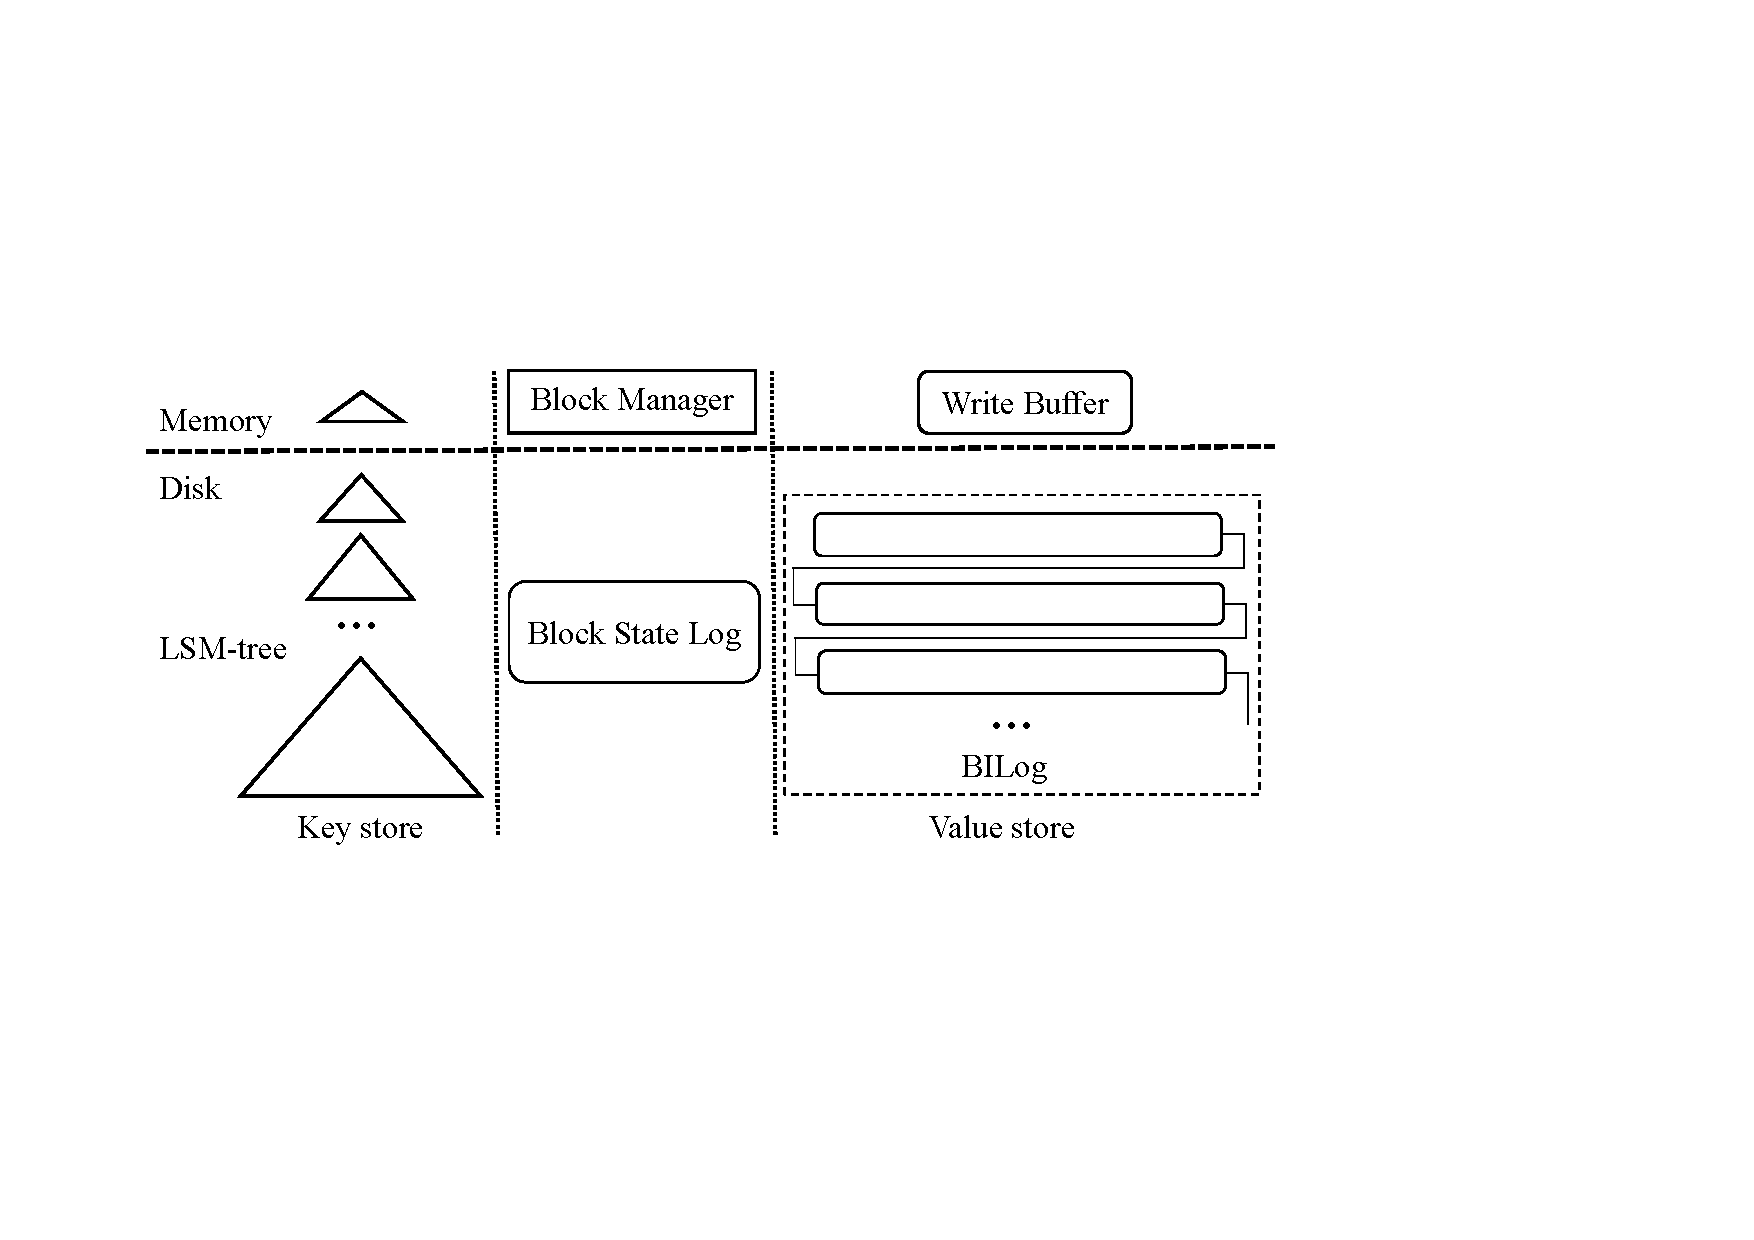
\includegraphics[width=90mm]{bikv.pdf}}
	\caption{BIKV architecture.}
	\label{fig:bikv}
\end{figure}

%失效块管理
\subsection{Block Manager} \label{ss1}
%数据结构:2种失效offset版本控制策略:频繁GC和update前提下失效offset版本控制和普通负载下
%块粒度
%失效块和有效块
%细节模块的实现以及实验中遇到的问题,对于更新密集或非密集情况下,重用块状态的管理
We build a block manager to record the validity of KV pairs in blocks, which covers the whole storage space of the vLog. Initially, all KV pairs are valid. When there generate compactions in the LSM-tree, the block manager continuously collects the invalid offsets extracted from the discarded KV pairs during the compaction processes. In this section, we introduce the detailed implementation of the block manager.
%For update-intensive workloads, it discards a large number of stale KV pairs during a compaction process in the LSM-tree of KV separation stores. The value of the discarded KV pairs is the offset of the stale values in the vLog. We build an invalid block manager to collect the invalid offsets, manage them in blocks (a block that contains invalid offsets called an invalid block, otherwise is a valid block) and reuse the invalid blocks in batches.

\subsubsection{Block Granularity}
%防止SSD的碎片化,对齐4KB,选择KV size和4KB的最小公倍数***************管理粒度的描述需要再斟酌一下
%In this paper, we focus on observing the benefits of the in-place reusable vLog for the KV stores that separate keys from values under update-intensive workloads. Thus, we assume the size of KV pairs remains constant.
The first step of building the block manager is to determine the block size $BS$, which is the management granularity of the block manager. We align the block size to SSD page size to eliminate the fragmentation of SSD. Thus, we set the block size as the common multiple of SSD page size and KV size to align both the size of the SSD page and KV pair. For example, if SSD page size is of 4 KB and KV pair size is of 1 KB, the block size is set as 4 KB. 

\subsubsection{Offset State in the vLog}
%数据结构,包括2个状态位图,表示块重用前和重用后状态
%因为各个偏移所对应的KV对只有2种状态,有效或无效,因此,对于每一个块,使用位图来表示块内所有位置的状态。在确定块大小后,设计整个VLOG的块数,块内的偏移数,来构建块管理器
The block manager covers the whole storage space of the vLog $SS$. After determining the block size $BS$, we sequentially divide the vLog into segments in block granularity. The number of blocks $BN$ is acquired by dividing the storage space of vLog by the block size ($SS$/$BS$). We assume the KV pair size is fixed $KS$. Then, we acquire the number of KV pairs $KN$ in each segment by dividing the block size by the KV size ($BS$/$KS$), which means each block manages such number of offsets. We use the state of a offset to represent the state of the KV pair it mapped in the vLog in the following.

It is necessary to consider how to mitigate the memory cost of the block manager. We use two simple hashes to scale down the vLog space: 1) dividing the starting offset of a block by the block size as the new starting offset; and 2) executing modulo operation between an offset and the block size and dividing the result by the KV pair size as intra-block offset. Thus, a block consists of a starting offset and $KN$ intra-block offsets.
%The number of intra-block offsets in a block is .

There are only two states of the KV pairs in the vLog: valid or invalid, which means we can use the \textit{bool} type to identify the validity of KV pairs. Thus, we use the \textit{bitmap} for each block to record the state of the offsets that belong to the block, represented as \textit{vLog-offset\_s}. The length of a bitmap is $KN$. We use 0 (default value) as valid flag, and 1 as invalid flag. When collecting an invalid offset, we compute the starting offset to locate the block the offset belongs to, and compute the intra-block offset to mark the corresponded bit position in \textit{vLog-offset\_s} to 1. When finishing the recycling of a block in a GC process, we clear \textit{vLog-offset\_s} of the block and mark all positions to 0. When recycling a block, we only need to verify the validity of KV pairs at the offsets with a valid flag in \textit{vLog-offset\_s} of the block.

\subsubsection{Offset State in the LSM-tree}
The way of identifying the validity of KV pairs is the same as that in Wisckey. For an offset with the valid flag in \textit{vLog-offset\_s}, firstly query the key and extract the offset from the value in the LSM-tree, secondly compare the two offsets, if they are the same, representing the KV pair is valid, otherwise, is invalid. When recycling a block, after identified the validity of the offsets, the subsequent processes are various for different validity:
\begin{itemize}
	\item For an invalid offset, it means that the stale index in the LSM-tree has not been discarded. When reusing this block, we write a new KV pair at the offset in the vLog and insert an index with the new key to the LSM-tree. 
	\item For a valid offset, we rewrite the KV pair to the vLog and insert an index with the new offset to the LSM-tree, resulting in that the former index in the LSM-tree becomes stale. 
\end{itemize}
%If an offset is verified to be invalid If an offset is verified to be valid, we rewrite the KV pair to the vLog and insert a KV pair with the new offset to the LSM-tree, resulting in that the former KV pair in the LSM-tree becomes stale. 
%The two situations both indicate that

No matter how, it results in that the offset emerges twice or even more at the same time in the LSM-tree, which arouses a severe problem of consistency: when the stale version of the offset is discarded in the LSM-tree, it marks the offset as invalid; but actually, currently the KV pair at that offset is valid. If the block is recycled later, it results in data loss within the block. In other words, we can find the key in the LSM-tree, but the KV pair at the offset in the vLog does not match the key. To resolve this problem, we have to record the offsets which have multiple versions in the LSM-tree.

The frequency of compaction in the LSM-tree and of GC in the vLog affect the existence of offset versions. We first assume there are at most two versions of an offset in the LSM-tree. Thus, we use another bitmap for each block to record the states of offsets in the LSM-tree, represented as \textit{LSM-offset\_s}. Similarly, 0 (default value) represents a valid flag (i.e., only one version), and 1 represents an invalid flag (i.e., existing two versions of the offset). When recycling a block in a GC process, corresponding to the positions with a valid flag in \textit{vLog-offset\_s} of the block, we mark the same bit positions to 1 in \textit{LSM-offset\_s}. When collecting an invalid offset which has an invalid flag in \textit{LSM-offset\_s} of the block it belongs to, we discard the offset directly and mark the bit position to 0.

%重新画图,4位为例,2个阶段,GC前,GC后
%In summary, the data structure of the states of a block (ie, the metadata) in the block manager consists of two bitmaps, representing the state of offsets in the vLog and the LSM-tree, respectively. 
There is an example of the two state bitmaps of a block, as shown in Fig.~\ref{fig:iblock}. The length of the bitmap is 4. Before recycling the block, \textit{vLog-offset\_s} of the block accumulates 3 invalid flags, and only the first offset is valid, while the states in \textit{LSM-offset\_s} are all valid. When recycling the block in a GC process, the states in \textit{vLog-offset\_s} assist In realizing a lightweight GC. After finishing the recycling of the block, correspondingly, the first position in \textit{LSM-offset\_s} is set as 1, while \textit{vLog-offset\_s} is cleared and the states are set as 0. The memory cost of the two bitmaps is negligible. For example, it costs 2 bits for each offset, if the storage space of vLog includes 1 billion offsets, the memory cost is about 239 MB.

%12.9 36MB的更新标注zifian分布
\textbf{Note that}, we do extensively experiments to verify the validity of \textit{LSM-offset\_s} for the consistency problem resulted by the multi-version offset in the LSM-tree. We find that under update-intensive workloads when it triggers GC intensively, there exists a situation that some blocks are frequently reused, which arouses a few multi-version offsets in the LSM-tree, resulting in data loss. For example, the experiment with 1 KB-KV pair and 4 KB-block, performed 40 M inserts, 36 M updates which follow a heavy-tailed Zipf distribution, and 40 M reads in order, generates several three-version offsets and results in 70 KV pairs lost. In this case, we change the bool state to counting state, which guarantees the consistency but costs more memory. When the bock size increases to 8 KB or even larger, using \textit{LSM-offset\_s} can guarantee consistency.

%失效块状态图
%Invalid status tables for each block in Invalid Block Manager
\begin{figure}[!t]
	\setlength{\abovecaptionskip}{0.cm}	
	\setlength{\belowcaptionskip}{-0.cm}
	\centerline{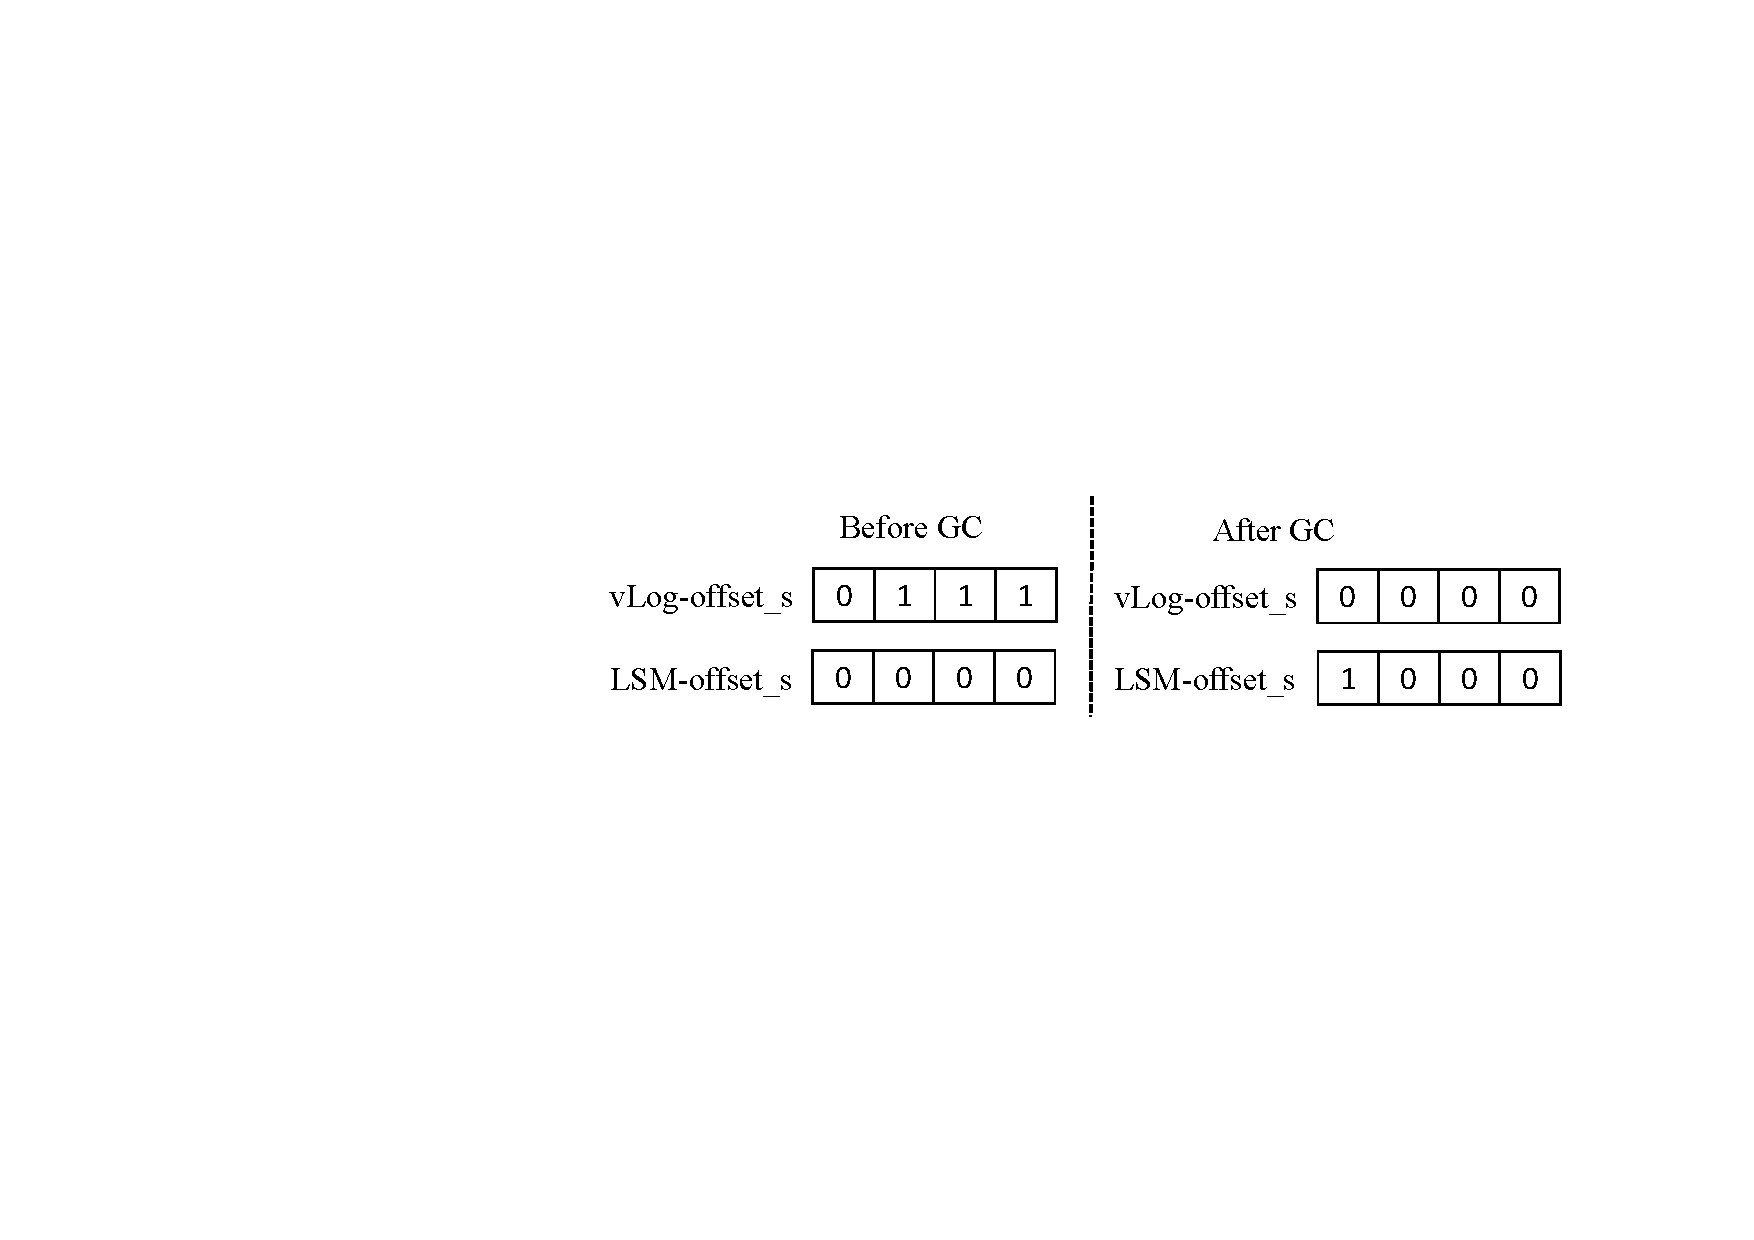
\includegraphics[width=80mm]{bitmap.pdf}}
	\caption{An example of two state bitmaps of a block.}
	\label{fig:iblock}
\end{figure}

\subsubsection{Block Classification}
As continuously accumulating invalid offsets, there exist three types of blocks based on the states in \textit{vLog-offset\_s} of a block, which have individual recycling processes, as follows: 
\begin{itemize}
	\item Entirely invalid block: the states are all invalid; when recycling such a block, directly clear the states in \textit{vLog-offset\_s} of the block;
	\item Invalid block: part of the states are invalid; when recycling an invalid block, firstly verify the validity of the KV pairs corresponding to the valid flags in \textit{vLog-offset\_s} and mark these positions in \textit{LSM-offset\_s} as 1, secondly rewrite the valid KV pairs to the vLog and insert the indexes to the LSM-tree, thirdly clear the states in \textit{vLog-offset\_s} and set them as 0;
	\item Valid block: the states are all valid; such blocks will not be recycled.
\end{itemize}

In BIKV, we design a priority to recycle the blocks based on the states in \textit{vLog-offset\_s} of each block, i.e., entirely invalid block $>$ invalid blocks with more than a half invalid flags (called half invalid block) $>$ other invalid blocks. This specification minimizes data rewrites and reduces the number of point queries in the LSM-tree, but meanwhile probably results in large amounts of access to the vLog. The blocks with high priority are usually less and probably distribute randomly. Thus, we buffer the starting offsets of the entirely invalid blocks and half invalid blocks in sorted order to save the iterating time for locating them and reduce accesses to the vLog at the cost of memory space, represented as \textit{buffer\_eib} and \textit{buffer\_hib}, respectively. For the invalid blocks, we set a pointer $pointer\_ib$ to loop the whole blocks in the block manager.

Generally, the GC unit size is larger than the write buffer size. Thus, we also buffer the starting offsets of the blocks recycled in a GC operation, represented as \textit{buffer\_rb}. For the entirely invalid blocks, directly insert them in \textit{buffer\_rb} when it triggers a GC operation. The memory cost of these buffers is negligible and varies under different block sizes and KV pair sizes. 

\subsubsection{Block State Log}
%用编码和解码的方式持久化状态,或直接按01持久化
We persist the states in \textit{vLog-offset\_s} and \textit{LSM-offset\_s} of blocks in the block manager to the block state log, aiming to recover the KV store and recover the indices not inserted into the LSM-tree during a GC operation when there is a crash. The states of blocks are changed in three operations: compaction in the LSM-tree, GC in the vLog, and reusing the available blocks. During a compaction operation, the block manager gathers invalid offsets from the values of the discarded KV pairs in the LSM-tree, and the states in \textit{vLog-offset\_s} of some blocks are changed. In a GC operation, the states in \textit{LSM-offset\_s} of the recycled blocks are modified. When reusing the blocks in \textit{buffer\_rb}, the states in \textit{vLog-offset\_s} of these blocks are set as 0. Thus, after finishing these operations, we persist the states in the corresponding bitmap of the blocks to the block state log.  

%We design a priority to select the candidate blocks in a GC operation based on the states in \textit{vLog-offset\_s} of each block
%Each block is mapping to a continuous segment in vLog. The data structure of each block consists of the starting offset (i.e., )
%The size of the offsets extracted from the KV pairs in the LSM-tree is 8 B. 
%locate the block and intra-block location according to a invalid offset  
%块重用
\subsection{Implementation of BILog} \label{ss2}
%失效块状态:全失效和部分失效,全失效块主动重用,部分失效块被动重用,半失效块重用时需要GC
%设计冷热区域vlog,预留部分写入GC数据,主区域写入后续的新数据
%数据flush时路径选择算法
%flush数据位置选择器,写个算法:主动重用和被动重用
%新:BILog的capacity是触发GC的容量,指热数据的能力,会预留一些空间放GC后的冷数据,预留空间不足时,把数据写入热区域
Based on the block manager, we design a block-conscious in-place reused vLog (BILog). We reclaim the space of vLog in blocks. When flushing the write buffer, we write the KV pairs to several blocks sequentially or randomly according to the available blocks, i.e., sequential write before starting to trigger GC and sequential/random write on recycled blocks. Generally, the size of valid KV pairs left in a GC process (which we consider as \textit{cold data}) is not aligning to the block size. To eliminate the fragmentation of blocks, we write the valid KV pairs to a separate region in the vLog called \textit{reserved space}, which meanwhile realizing the separation of hot/cold data. Thus, the storage space of the vLog is divided into two parts: a large piece for new data and a small piece for cold data, called main space and reserved space, respectively. We call the size of the main space as the capacity of vLog. When the data volume accumulates to the capacity of vLog, BIKV starts to trigger GC.

In BIKV, the valid range of vLog is always from 0 to the \textit{tail} (i.e., the pointer points to the current end of the vLog). The data always appends to the tail. Before thoroughly filling the main space, the new KV pairs append to the tail in the main space. After that, the valid KV pairs left in GC operations append to the tail in the reserved space. Whenever the position of the tail changes, we insert the tail and its offset into the LSM-tree in the form of tuple \textless `tail', offset \textgreater. There is an example of the data organization in BILog, as shown in Fig.~\ref{fig:ipbrLog}. The shadow positions indicate the invalid values, and the dotted box represents the data range of a block. The tail points to a position in the reserved space. Before that, the vLog is filled with KV pairs.  
%the reclaiming invalid blocks 

\begin{figure}[!t]
	\setlength{\abovecaptionskip}{0.cm}	
	\setlength{\belowcaptionskip}{-0.cm}
	\centerline{\includegraphics[width=80mm]{vLog.pdf}}
	\caption{Data organization in BILog.}
	\label{fig:ipbrLog}
\end{figure}

\subsection{Garbage Collection} \label{ss3}
%当BILog累积到阈值大小时就开始触发GC,开始触发GC后,根据可用块池中的块的大小是否大于buffser size来决定要不要GC,GC单位是块大小和写缓冲的公倍数
Garbage collection is indispensable to reclaim the space occupied by invalid values in the vLog. In BIKV, GC operates in units of an integer multiple of block size $GC_u$ (e.g., 64 MB), and is triggered when the capacity of vLog is running out. We design a lightweight GC strategy with the aid of the block manager, and overall, a GC operation is to recycle the blocks with invalid flags. The number of blocks recycled in each GC $GC_bn$ is acquired by dividing the GC unit size by the block size.

In BIKV, if it finds that the tail is at the end of the main space or moved to the reserved space when flushing the write buffer, it starts to trigger GC. At the beginning of GC, we poll the blocks according to the priority to select the candidate blocks and then recycle these blocks. The process is shown in Algorithm~\ref{alg:gc}.
%GC策略写一个算法 
%When it starts to trigger GC, if the total size of the entirely invalid blocks is more than the GC unit size (e.g., 64 MB default), we directly clear the states in \textit{vLog-offset\_s} of these blocks and flush the KV pairs in the write buffer to these blocks subsequently. If the entirely invalid blocks are running out (i.e., the size of the left blocks is less than GC unit size), it starts to recycle the blocks.
\begin{algorithm}[htbp]
	\caption{The process of a GC operation}
		\begin{algorithmic}[1]
			\IF{There exists entirely invalid blocks}
			\STATE Insert the blocks in \textit{buffer\_eib} to \textit{buffer\_rb}; 
			\ENDIF
			\IF{The total size of the blocks in reusable block pool is larger than the write buffer size} 
			\STATE Do nothing;
			\ELSE
			\IF{There exists half invalid blocks} 				
			\IF{The total size of these blocks is larger than GC unit size}
			\STATE Get $GC_bn$ blocks from \textit{buffer\_hib};
			\ELSE
			\STATE Get all half invalid blocks from \textit{buffer\_hib};  
			\STATE Get the rest number of invalid blocks by looping the block manager with $pointer\_ib$;
			\ENDIF
			\ENDIF
			\STATE Reclaim the candidate blocks and insert them to \textit{buffer\_rb};
			\ENDIF
		\end{algorithmic}
	\label{alg:gc}
\end{algorithm}

After finishing the GC operation, we flush the write buffer to the available blocks in \textit{buffer\_rb}. Overall, when flushing the write buffer to the vLog, we should select the write location according to the tail. The algorithm of the write location selection for flushing is shown in Algorithm~\ref{alg:reuse}. When the write buffer is full, it flushes the data to the vLog. The first step is to judge the position of the tail. If the tail is in the main space, directly append data to the tail of vLog. Otherwise, it determines whether to trigger a GC operation based on the number of blocks in \textit{buffer\_rb}. 

\begin{algorithm}[htbp]
	\caption{Write location selection algorithm for flushing}
	\begin{algorithmic}[1]
		\STATE Get the tail of vLog; 
		\IF{The tail is in the main space} 
		\STATE Append data to the tail of the vLog;
		\ELSE
		\IF{The total size of blocks in \textit{buffer\_rb} is more than the write buffer size}
		%\COMMENT{All values in the segments managed by those blocks are invalid} %测试
		\STATE In-place update data to these blocks and erase them from \textit{buffer\_rb};
		\ELSE
		\STATE Trigger a GC operation; 
		\STATE In-place update data to the available blocks and erase them from \textit{buffer\_rb};
		\ENDIF
		\ENDIF			
	\end{algorithmic}
	\label{alg:reuse}
\end{algorithm}
 
% This rule has a complex impact on GC overhead because it reduces the number of KV pairs which need to identify the validity (i.e., point queries) in the LSM-tree, but probably results in large amounts of access to the vLog.
%Based on the invalid block manager, we design two invalid block reuse policies: a positive reuse policy and a negative reuse policy. The positive reuse policy is to actively reclaim the entirely invalid blocks (i.e., the invalid offset bitmap of vLog in a block is all set to 1) before the size of vLog accumulating to a threshold, aiming to mitigate management overhead and save storage space. The positive reuse policy is triggered when flushing KV pairs in the write buffer to the vLog. The negative reuse policy is to passively reclaim the invalid blocks after the volume of values in vLog accumulating to a threshold. It is triggered in the process of garbage collection to discard the stale values and release storage space.
%When reusing a block, we iterate through the invalid offset bitmap of vLog, for the position whose value is 0, we query the LSM-tree to check the validity of the KV pair. If the offset is stale for that key in the LSM-tree, we set the corresponding position in the invalid offset bitmap of the LSM-tree to 1. 
%When the data in vLog accumulates to a threshold, it starts to trigger GC. The process of GC is lightweight with the help of the invalid block manager. First, based on the invalid offset bitmap of vLog in each block, acquire a specific volume of blocks (e.g., 64MB) in which the number of invalid offsets accounts more than others. Second, read the KV pairs in those blocks except the entirely invalid blocks. Third, find which of those values that corresponding bit position are 0 are valid by querying the LSM-tree. Finally, append valid values back to the vLog and modify the invalid offset bitmap of vLog in these invalid blocks to be 0. Subsequently, we flush new data to the GCed invalid blocks. 

%\subsection{In-place Block Reusable vLog}
%对于被动重用的操作,我们将vlog分为可用部分和预留部分,主要有2个好处:解决被动重用中有效数据的写对齐问题;将GC后的有效数据(相对冷数据)写到预留位置,如图所示
%In IpBrKV, the value log is an in-place reuse vLog. Since the vLog is recycled based on blocks, we call it in-place block-reusable vLog. For the negative reuse in IpBrKV, it triggers GC operations, resulting in valid data in the reclaiming invalid blocks be rewritten. To simplify the block management, we divide the vLog into available part and reserved part. The new data is always written into the available part; while the valid data produced in GC operations is rewritten into the reserved part. There are two benefits to this distribution: (1) avoid the problem of write alignment caused by rewriting the valid data into the reusable blocks; (2) realize separation of hot and cold data, because the valid values rewritten in GC operation are relatively cold data. There is an example of the data status of the two parts in in-place block-reusable vLog, as shown in Fig.~\ref{fig::ipbrLog}. The shadow positions indicate the invalid values, the Dotted box represents the data range that a block maps to.

\subsection{Recovery} \label{ss4}
%基于Wisckey的foundation,拥有其相关的一致性方案,如容忍缓冲数据丢失,key store的一致性,由于采用就地块重用技术,因此将writefront和in-place update block offset持久化到LSM-tree,同时,为了支持可恢复,添加失效块状态日志,就如同LevelDB中的version的持久化一般持久化失效块状态,每次compaction后持久化当前失效块管理器中存在失效偏移量的各失效块状态
%
The recovery methods of BIKV are different from those of Wisckey because of BILog. If there happens a crash, the recovery process of the indices in the key store includes two steps. First is the recovery in the LSM-tree, i.e., scanning the write-ahead log after reboot to recover unpersisted KV pairs. Second is the recovery of the bulk indices not inserted into the LSM-tree during flushing the write buffer or GC in the vLog, i.e., getting the offset of the tail from the LSM-tree and scanning the vLog starting from the offset, if there exist data, get the key and offset, and keep forward scanning till the end, finally insert the indices to the LSM-tree; otherwise, getting the offset of the last inserted non-tail key from the LSM-tree, scanning the block state log until finding the block that offset belongs to, and keeping scanning to get the offset of the reused blocks till the end, finally inserting the indices of the KV pairs in those blocks to the LSM-tree.

It is necessary to recover the states of blocks in the block manager; otherwise, BIKV degenerates to Wisckey at initially recovered until accumulating a number of invalid offsets again. We recover the states by scanning the block state log till the end.

%\subsection{Limitations}
%由于是就地更新,因此应用场景有约束,适用于固定KV大小的应用或大部分大小相近(会产生少量的空间浪费),本文中的实验使用固定的KV进行,对可变KV大小的支持可后续研究
%KV size,较坏情况下,失效的块不连续,面临着产生大量随机读写的问题,在SSD下随机读写和顺序性能相关不大,但是IO次数变多仍然会有影响
%In summary, there are several limitations for the block-conscious in-plate update
%In a worse case that the invalid blocks are discontinuous, it results in large amounts of random reads and writes. Although the difference between the sequential and random performance is not significant, the large number of I/Os has a negative impact on the system. 
%Intuitively, the nature of in-place reuse makes BIKV not suitable for the applications in which the size of KV pair is variable. In this case, it makes the invalid block management more complicated and will result in a certain amount of space waste. In this paper, we focus on observing the benefits of the design of in-place reuse in blocks under update-intensive workloads. Thus, we assume the KV size remains fixed to simplify the design of the invalid block manager.

\section{Evaluation} \label{sec4}
%写放大,空间放大,写性能,读性能
%不同大小的KV pairs的写放大,空间放大,写性能,读性能
%Wisckey,hashkv的预留空间不同(GC少)时,三者的性能
%LSM-tree中产生的compaction的数量,分析compaction对写性能的影响,建议采用compaction优化的LSM-tree
%就地更新所产生的随机写在HDD上的影响
In this section, we do a set of experiments to compare BIKV with widely-used and state-of-the-art LSM structured and KV separated KV stores, including LevelDB \cite{LevelDB}, HyperLevelDB \cite{HyperLevelDB}, PebblesDB \cite{PebblesDB}, Wisckey \cite{Wisckey} (i.e., vLog implementation in the prototype of HashKV) and HashKV \cite{HashKV}. We evaluate the KV separation stores with the testbed in HashKV which generates workloads using YCSB \cite{YCSB}, and evaluate LSM-based KV stores using the microbenchmarks (\textit{db\_bench}). For fair comparison, we replace the key generator in \textit{db\_bench} with that in the testbed to produce the same workload. The evaluation results attempt to answer the following questions:
\begin{itemize}
	\item How is the write and read performance of BIKV compared to other KV stores under mixed write/read workloads?
	\item How is the write amplification and performance of BIKV compared to other KV stores under GC-intensive workloads with various KV pair sizes?
	\item What is the impact of GC strategies and the number of GC on the three  KV separation stores under various GC timing?  
	\item What is the impact of management granularity on BIKV?
\end{itemize}

\subsection{Experimental Setup}
%是否用一个表表明各KV store参数?
The evaluation is performed on an Intel Xeon E5-2609v2 2.5 GHz processor with two cores, 32 GB of RAM, running 64-bit Centos 7.2 with the Linux 3.10 kernel. The xfs file system is run on top of a 480 GB SSD (ATA GALAX GXTA1C0480). 

\begin{table}[!t]
	\setlength{\abovecaptionskip}{0.cm}	
	\setlength{\belowcaptionskip}{-0.cm}
	\centering
	\renewcommand\tabcolsep{4pt}
	\renewcommand\arraystretch{1.1}
	\caption{Parameters of the six KV stores}
	\label{tab:p}
	\scalebox{0.8}{
		\begin{tabular}{cccccc}
			\hline
			 & \textbf{KV stores} & \textbf{MT} (MB) & \textbf{SST} (MB) & \textbf{BF} (b/k) & \textbf{GC unit} \\
			\hline
			 & \textbf{LDB} & 32 & (4,16,32) & 10 & -\\
			LSM & \textbf{HDB} & 32 & default & 10 & - \\
			structured & \textbf{PDB} & 32 & default & 10 & - \\
			\hline
			 & \textbf{Wisckey} & 4 & (2,4) & - & 64 MB\\
			KV & \textbf{HashKV} & 4 & (2,4) & - & segment group\\
			separated & \textbf{BIKV} & 4 & (2,4) & - & 64 MB \\
			\hline
		\end{tabular}
	}
\end{table}

The important parameters of the six KV stores, LevelDB (\textbf{LDB}), HyperLevelDB (\textbf{HDB}), PebblesDB (\textbf{PDB}), Wisckey, HashKV, and BIKV are shown in Table \ref{tab:p}. The larger size of Memtable can improve the write performance \cite{OHDB, FloDB}. The larger size of SST can improve the read performance \cite{OHDB}. In HashKV, a segment group includes a main segment (64 MB) and several log segments (1 MB). In LevelDB, the size of SST increases with the size of KV pairs. Besides, in the LSM structured KV stores, we turn off the data compression since there is no data compression in the KV separation stores. For other parameters, such as the threshold size of each level, we use the default values in the experiments. For the KV separated KV stores, we use LevelDB as the key store. The size of write buffer is set to 1 MB. We use the hotness awareness extension for HashKV which can improve the write performance and reduce write amplification. 

The size of KV pairs is fixed, such as 1 KB, including the 8 bytes metadata (consisting of sequence number and type in LSM structured stores or key/value size in KV separated stores), 24 bytes key, and 992 bytes value. We use multi-step single-threaded microbenchmarks to observe the write and read performance, performing 40 M inserts (about 39 GB of data, resulting in about 1.9 GB of key store in KV separation stores), four rounds of 12 M updates (about 12 GB of data, resulting in about 0.78 GB of key store) following a heavy-tailed Zipf distribution and two rounds of 40 M reads. The seven-step operation is Load, Update \#1, Update \#2, Read \#1, Update \#3, Read \#2, Update \#4 in turn. 
%In the load step, it performs 40 M random writes (about 39 GB of data, resulting in about 1.9 GB of key store in KV separation stores). In each update step, it performs 12 M updates (about 12 GB of data, resulting in about 0.78 GB of key store) following a heavy-tailed Zipf distribution. In each read step, it performs 40 M random reads.

\subsection{Performance Comparison}
%键值分离存储中LSM-tree部分采用的是默认参数的实验结果;之后的实验中SST的大小改为4MB
This section evaluates the write and read performance of the six KV stores. We use the default parameters of the LSM-tree in KV separated stores where the SST size is of 2 MB, while in other sections, we set the SST size as 4 MB to accelerate the experiments. We fix the size of each KV pair as 1 KB. In the experiments, we observe that after performing all the steps, the size of maximum space amplification of LevelDB, HyperLevelDB, and PebblesDB is about 63 GB, 51 GB, and 63 GB, respectively. Thus we set the capacity of Wisckey, HashKV and BIKV to be 58 GB (i.e., all of them start to trigger GC when the size of vLog accumulates to 58 GB). In HashKV, we set the main segments of 40 GB and the log segments of 18 GB. 
% In HashKV, it starts to trigger GC when the reserved space is running out while Wisckey and BIKV start to trigger GC when they fills up the vLog.

The experimental results are as shown in Fig.\ref{fig:pc}. We can observe the write performance of random write, intensive update and write after read, as well as the read performance. Note that the KV separated stores start to trigger GC in Update \#2.

\paragraph*{Random write}
%随机写,基本没有或较少update 
In Load, it performs 40 M random writes. The write throughput of BIKV is close to Wisckey, and much better than the other four KV stores. In Update \#1, it performs 12 M updates immediately. The write throughput of Wisckey and BIKV also better than others, but significantly degrades. It may be affected by the compactions in the LSM-tree. 
%HashKV has lower write performance than Wisckey in the load phase because of its complex segment management. 

\paragraph*{Intensive update}
In Update \#2, the KV separated stores start to trigger GC. The write throughput of Wisckey and HashKV significantly degrades. The write throughput of BIKV also degrades, but is much better than others. In the last two update round, it becomes GC-intensive. Compared to the write throughput of HyperLevelDB and PebblesDB,  that of Wisckey is worse, that of HashKV is close to them, while BIKV is much better. BIKV benefits from the previously accumulated invalid offsets.  

\paragraph*{Random read}
The read throughput of the KV separated stores is better than LevelDB and HyperLevelDB because of the much smaller key store (more than 25 X), although they need an additional access to vLog. The read throughput of BIKV is close to Wisckey and better than HashKV. HashKV may be affected by an additional access to cold data log.

\paragraph*{Write performance after read}
%读后写性能,可见compaction对KV分离存储的影响,结论:选用优化的LSMs
We set two round intensive read among intensive write to (1) acquire the read performance, and (2) observe the write performance after intensive read, in other words, observing the impact of compactions. We find that the write throughput of LevelDB and HyperLevelDB significantly improves in Update \#3 and \#4. For the KV separated stores, they trigger GC frequently in both Update \#3 and \#4. But the write throughput of BIKV and Wisckey in Update \#4 is significantly better than that in Update \#3, while that of HashKV only has a little improving. The reason is that in the LSM-tree, intensive read arouses a number of \textit{seek\_compaction} and emptys the space of upper levels, thus mitigating the impact of compactions to the write performance.
%It shows that the read step before Update #4 has a positive effect.

\begin{figure}[!t]
	\setlength{\abovecaptionskip}{0.cm}	
	\setlength{\belowcaptionskip}{-0.cm}
	\centering
	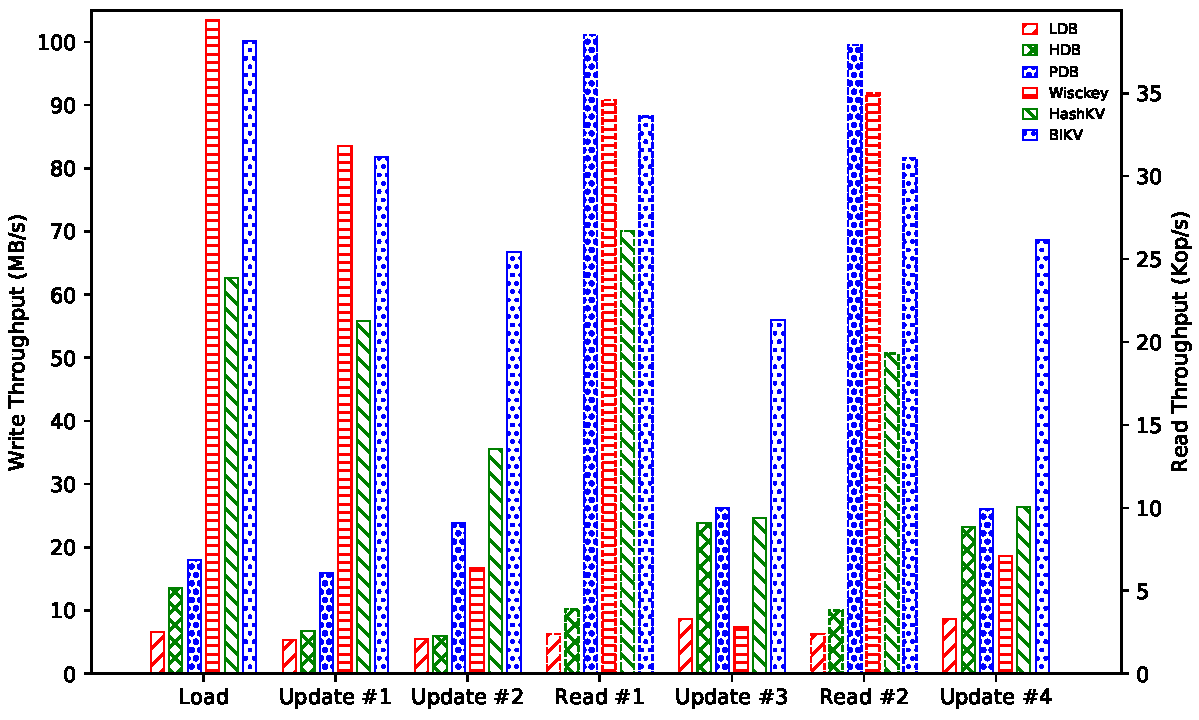
\includegraphics[width=80mm]{total_performance.pdf}
	\caption{The performance of 6 KV stores under 7 steps.}
	\label{fig:pc}
\end{figure}

\subsection{Impact of KV Size}
% 块管理粒度为128KB,GC阈值设计为第一次update的一半,从密集GC的角度观察性能
%KV size较小时,对于键值分离存储,元数据与数据大小接近,即LSM-tree中的数据(key,offset)和vLog中的数据(keysize,valuesize,key,value)的size相差倍数不大,使得键值分离存储具有明显劣势:1.数据需要写2份,写开销增加近一倍;2.空间开销大,且会造成较大的写放大;键值分离存储比LSM-based存储在KV size小时性能差,当size大于1KB时性能好,已经在其他工作中得到证明 \cite{Wisckey, HashKV}。在这一节,我们主要观察三种键值分离存储对于不同KV size的性能。
We study the performance of KV stores under various KV pair sizes which vary from 256 B to 16 KB. Specifically, we adjust the KV pair size by only changing the value size and keeping the key size fixed at 24 B. We maintain the number of KV pairs loaded or updated to acquire the performance of KV stores under the same order of magnitude operations. We reduce the number of inserts/reads to 10 M and that of updates to 3 M when the KV size is 16 KB because of the limitation of SSD size. Thus, for the KV pair size of 4 KB and 16 KB, the total size of inserts and each round updates is 153 GB and 46 GB, respectively.

We set the capacity of KV separated stores as 45 GB that makes them start to trigger GC in Update \#1. In latter update steps, updates are issued to the fully filled value store and will trigger GC frequently, thus forms a GC-intensive workload. In BIKV, the block size is of 128 KB. The experimental results are as shown in Fig.\ref{fig:kv}. We can observe the write/read performance and write amplification under various KV pair sizes. 

%摘自hashKV
%We include both P2 and P3 to ensure that the update performance is stable. HashKV adds a separate region in the value store file for the cold data log.

\begin{figure} [!t]
	\setlength{\abovecaptionskip}{0.cm}	
	\setlength{\belowcaptionskip}{-0.cm}
	\centering
	\subfigure {
		\begin{minipage}{\linewidth}
			\centering
			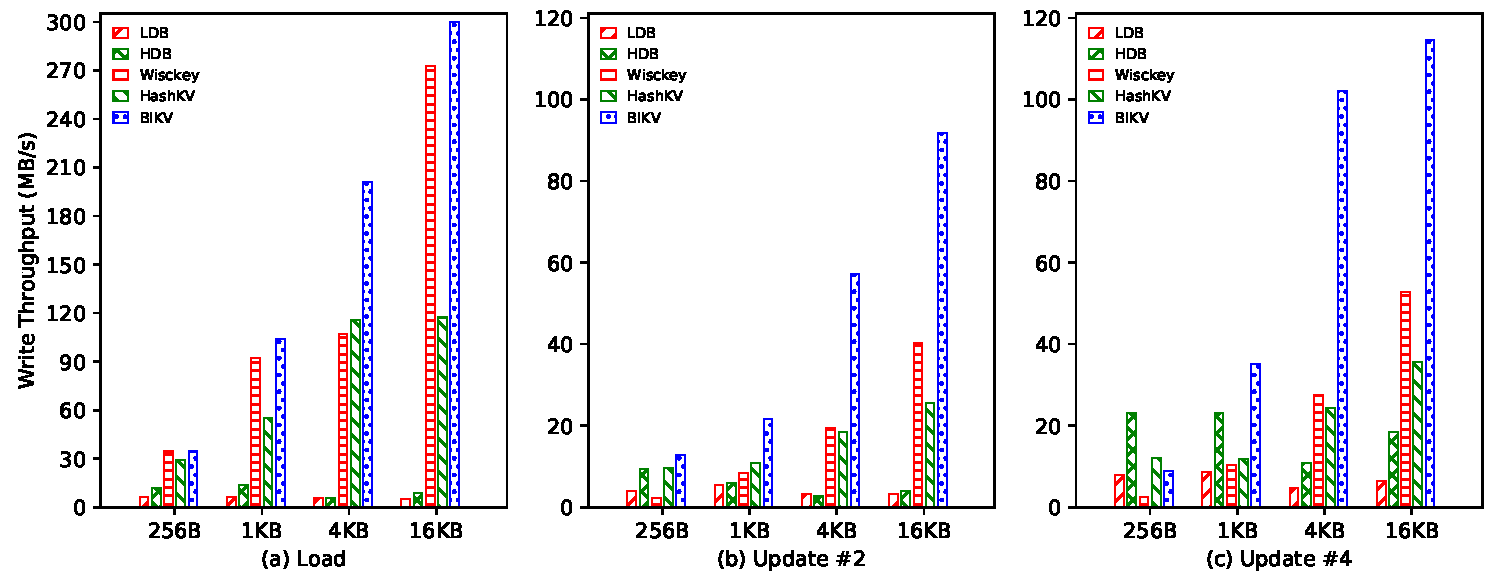
\includegraphics[width=85mm]{kvsize_wt.pdf}
		\end{minipage}
	}  	
	%\vfill
	\subfigure {
		\begin{minipage}[t]{0.31\linewidth}
			\centering
			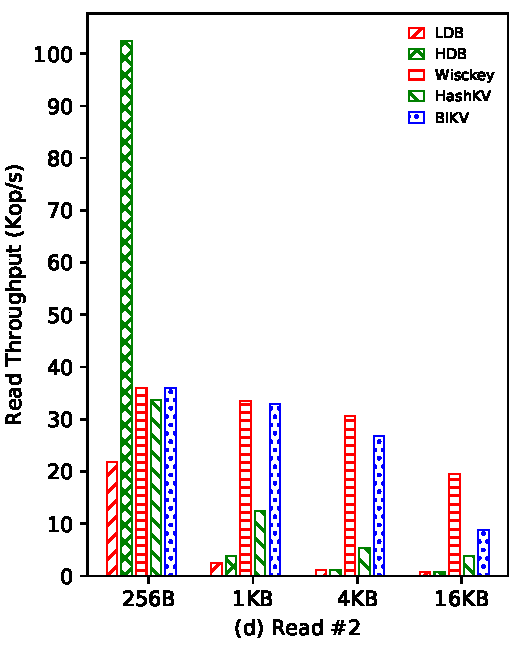
\includegraphics[width=27mm]{kvsize_r.pdf}
		\end{minipage}
		\hfill
		%\vspace{0.02cm}
		\begin{minipage}[t]{0.31\linewidth}
			\centering
			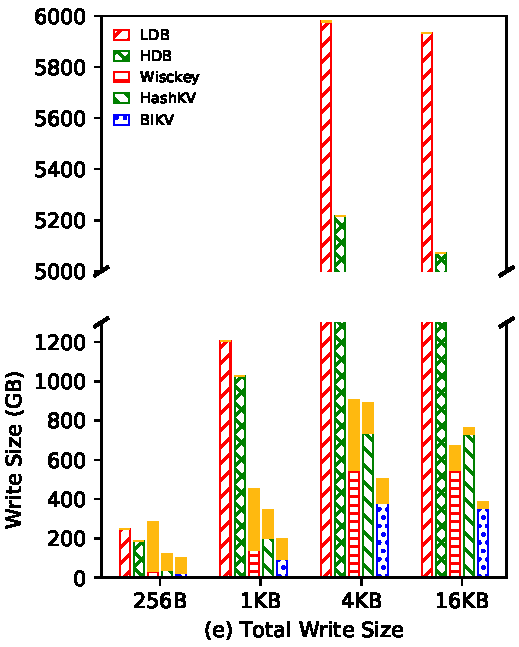
\includegraphics[width=27mm]{kvsize_tw.pdf}
		\end{minipage}
		\hfill
		%\vspace{0.02cm}
		\begin{minipage}[t]{0.31\linewidth}
			\centering
			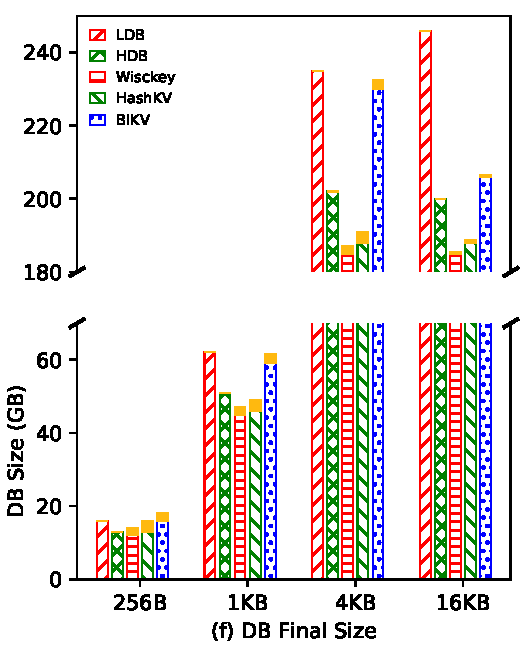
\includegraphics[width=27mm]{kvsize_fs.pdf}
		\end{minipage}
	}
	\caption{Experimental results of 5 KV stores under various KV pair sizes.}
	\label{fig:kv}
\end{figure}

\paragraph*{Write performance}
%load 和 update2的性能
We show the write throughput in Load, Update \#2 and Update \#4 of five KV stores under various KV pair size, to illustrate the write performance under random write, intensive GC and intensive update, respectively.

In Load, the write performance of BIKV is always the best, as shown in Fig.\ref{fig:kv} (a), and it is close to Wisckey when KV pair size is less than 1 KB. In Update \#2, the KV separated stores trigger GC intensively. The write performance of BIKV is also the best, as shown in Fig.\ref{fig:kv} (b), benefiting from the lightweight GC. In Update \#4, firstly, the write performance of the KV stores is improved, benefiting from Read \#2. Besides, up to Update \#4, KV separated stores have accumulated large volume of updates which mitigates the overhead of GC in Update \#4, resulting in better write throughput than that in Update \#2, as shown in Fig.\ref{fig:kv} (c).
%It can clearly be seen that the write throughput of the KV stores is better than that in Update #2 at most cases

\paragraph*{Read performance}
We show the read throughput of Read \#2 to illustrate the read performance of the KV stores under various KV pair sizes. As shown in Fig.\ref{fig:kv} (d), when the KV pair size is of 256 B, HyperLevelDB has the best read performance because of the less number of SST. The write performance of BIKV is close to that of Wisckey when the size of KV pair is less than 1 KB, while it is worse than Wisckey when the size of KV pair is larger than 4 KB. The reason might be the large random read caused by the in-place update.

\paragraph*{Write amplification}
%the difference in write amplification between NG-KV and other stores goes up as the number of keys increases. 
In the KV separated stores, the storage space consists of the key store and value store. We use the solid bar represents the size of the key store as shown in Fig.\ref{fig:kv} (e) and (f). We combine the size of cold data log and vLog for HashKV. 

The total write size of BIKV is always the least. For KV separated stores, when the KV pair size is less than 1 KB, the total write size of the key store is even larger than that of the value store, as shown in Fig.\ref{fig:kv} (e). The final size of BIKV is close to LevelDB at most cases and always larger than the other three as shown in Fig.\ref{fig:kv} (f), because it appends the valid data left in each GC to BILog. Write amplification (WA) is obtained by dividing the total write size by the total data size, e.g., when KV pair size is 1 KB, the data size of five rounds writes is about 84 GB. WA of LSM structured stores goes up as the KV pair size increases, e.g., it scales from 11.9 to 17.8 X in Wisckey. On the contrary, WA of KV separated stores goes down as the KV pair size increases. WA of BIKV is always the least, it degrades from 4.8 to 1.5 X.

%Corresponding to GC aroused in vLog and compaction aroused in the LSM-tree, we represent the number of GC and compaction in the form of "GC - C" in the column of total write. For HashKV, the cold data size in HashKV is 236MB.

\subsection{Impact of GC Timing}
%3个KV分离的store之间比较,观察密集GC和非密集GC的系统性能
We study the write performance of KV separated stores under various GC timing, i.e., the time to start to trigger GC. We set the capacity of value store as 45 GB and 60 GB to make the systems start to trigger GC in the middle of Update \#1 and late of Update \#2, respectively. The KV pair size is of 1 KB. In BIKV, the block size is of 4 KB aligning to the page size in SSD. The experimental results are as shown in Fig.\ref{fig:gc}. We found that various GC strategies have different impact not only on the number of GC and write performance but also on the total write size to the LSM-tree and vLog.

\begin{figure}[!t]
	\setlength{\abovecaptionskip}{0.cm}	
	\setlength{\belowcaptionskip}{-0.cm}
	\centering
	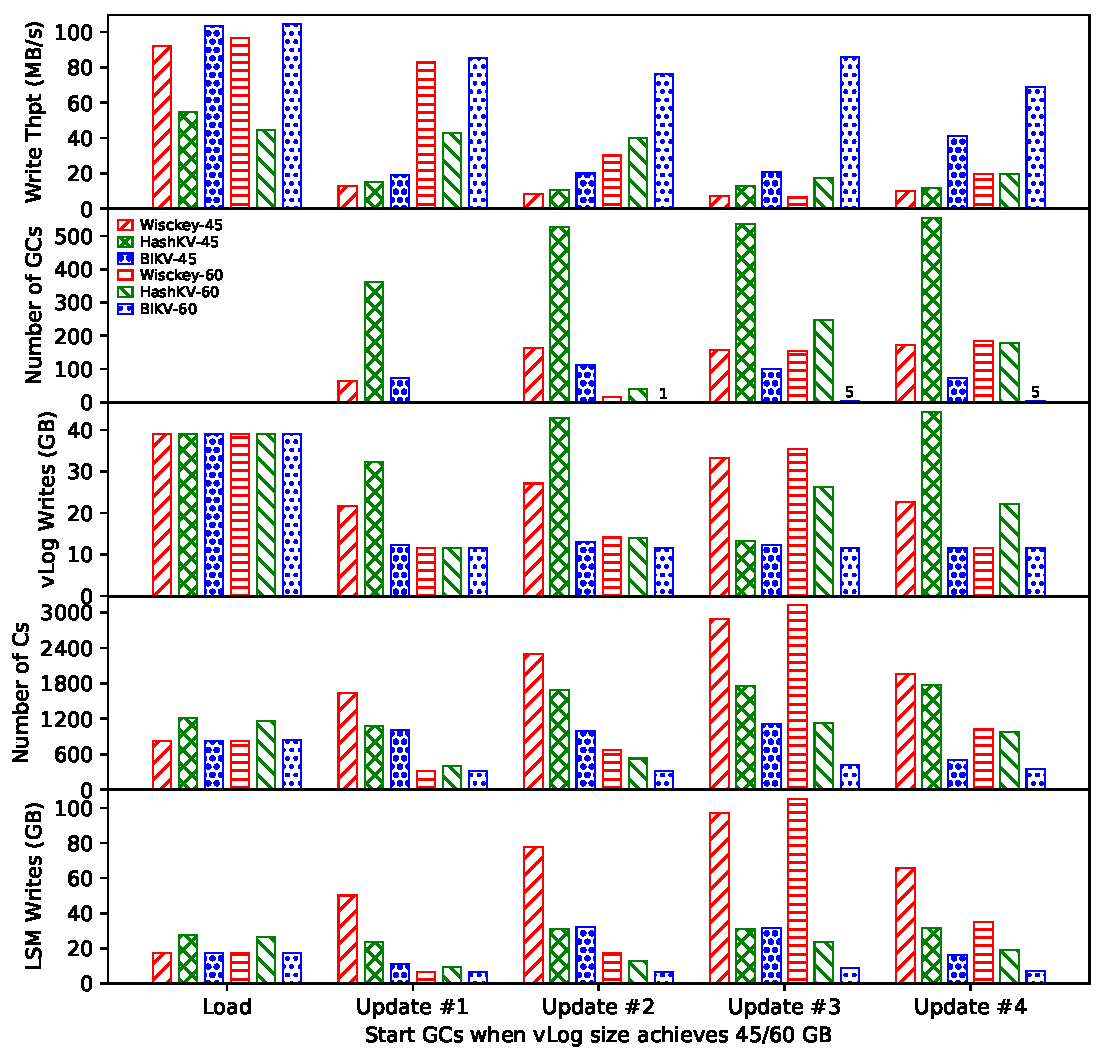
\includegraphics[width=90mm]{gc_timing.pdf}
	\caption{The detailed operations of the key store and value store under different GC timing.}
	\label{fig:gc}
\end{figure}

%密集GC时,不同的GC策略对LSM产生影响,compaction数量不同,写入的数据量不同,hashkv一次GC为一个segment group,大于64MB,带有cold data log
%hashkv因为固定size,所以产生大量GC,因为GC开销相对较小,因此对写性能影响不大
%vlog重写的量多,造成的C和LSM写入就多,写性能差
%BRKV GC较少,性能提升,C/LSM/VLOG都少
For the value store of 45 GB, it forms a GC-intensive workload. When it starts to trigger GC, the write throughput significantly decreases. Various GC strategies result in different amount and sequence of rewritten KV pairs, leading to different number of compaction and total write size in the LSM-tree. For example, in Update \#1, the number of GC in HashKV is the most, resulting in the largest total writes to vLog, but the number of compaction and total write size in the LSM tree is less than Wisckey. For BIKV, the number of GC is a little more than that in Wisckey, but the total writes to vLog, the number of compaction and total writes in the LSM-tree is the least. Generally, BIKV triggers the least GC, which mitigates the impact on write performance and leads to the least total writes to vLog and total writes to the LSM-tree.
%, and the write throughput is better than Wisckey because of the optimized GC

For the value store of 60 GB, before triggering GC frequently, the write throughput of Wisckey and BIKV keeps decreasing from Load to Update \#2, it illustrates that compactions in the LSM-tree have a negative impact on write performance. The total write size and number of compaction in the LSM-tree of HashKV are larger than that of Wisckey and BIKV because of the different sequences of KV pairs writing to vLog. Starting from Update \#3, it triggers GC frequently. BIKV has the best results in all respects, benefiting from the large amount of invalid offsets accumulated under update-intensive workload.


\subsection{Impact of Block Granularity}
%实验参数:45GB,1KB,实现密集GC,块粒度从4KB(对齐SSD 页)到1MB(对齐写buffer),以2的倍数增长进行了大量的实验,观察块粒度的影响
%分析数据发现是块粒度的选择是一个trade-off,块粒度较小时,一个块内key数量少,容易产生满块,但是由于GC时会选择失效KV较多的块,因此,容易产生大量随机读;而大粒度块内有效KV较多,因此GC时产生较多的读LSM的操作;其中,LSM读操作次数影响更多
%给出几个块粒度在U1-U4阶段的写性能(load阶段性能挖近似),同时在表中给出一组具有代表性的实验数据,是不同块粒度下U3阶段的写性能,GC数,在value log上进行的读操作和LSM中进行的查找操作,来观察不同块粒度对GC及写性能的影响。
We study the impact of block granularity on BIKV. The block size varies from 4 KB to 1 MB (aligns to the write buffer). We set the capacity of value store as 45 GB. The KV pair size is of 1 KB. The write throughput of BIKV with various block sizes under four round updates is as shown in Fig.\ref{fig:bg}. We found that it is a trade-off to determine the block size. We illustrate the experimental results in Update \#1 and Update \#3 (as shown in Table \ref{table:bg}) as examples to describe the reasons. \textbf{WT}, \textbf{GCs}, \textbf{BILog-Rs} and \textbf{LSM-Rs} stand for write throughput, the number of GC, the number of read access to BILog and the number of reads in the LSM-tree, respectively.

\begin{figure}[t]
	\setlength{\abovecaptionskip}{0.cm}	
	\setlength{\belowcaptionskip}{-0.cm}
	\centering
	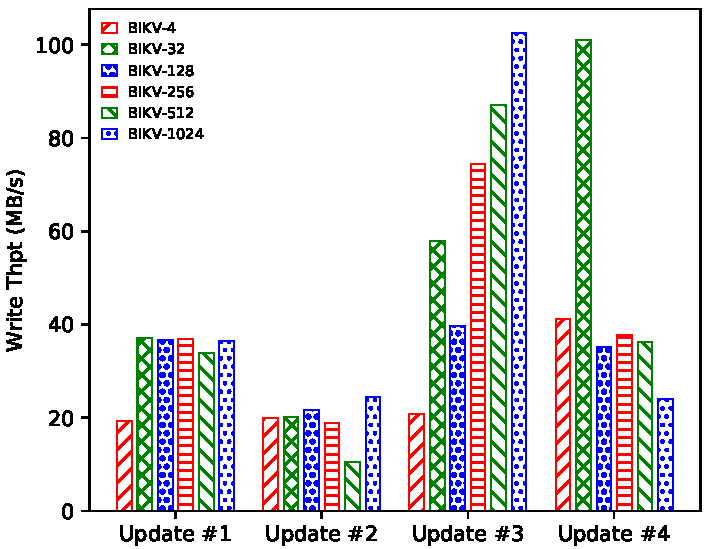
\includegraphics[width=80mm]{block_gra.pdf}
	\makeatletter\def\@captype{figure}\makeatother\caption{Write performance of BIKV under various block sizes.} 
	\label{fig:bg}			
\end{figure}

As shown in Fig. \ref{fig:bg}, the write throughput is relatively stable when the block size of BIKV is 32 KB (32 KB-block). The write performance of 1 MB-block benefits from one write access to BILog when flushing the write buffer. The effect of block size on the write performance of BIKV is not intuitive. Theoretically, smaller block includes less number of KV pairs, thus it is easier to accumulate entirely invalid blocks. However, since BIKV prefers to recycle the invalid blocks with more invalid flags, it would lead to many and random accesses to BILog in each GC. On the contrary, for the larger block, it is hard to accumulate many invalid Offsets in each block, thus it is more likely to arouse a few visits to BILog in each GC. However, it would generate more reads to the LSM-tree because of less invalid flags. In short, the cost of smaller block size is on multiple access to BILog while larger blocks size costs a lot on large amount of random reads to the LSM-tree.

In Update \#1, BIKV starts to trigger GC. The number of GC is 74 under all the block size. The number of read access to BILog and the number of reads to the LSM-tree aroused by GC is (1.2 M, 1.9 M) under 4 KB-block and (74, 3.4 M) under other block size, respectively. The difference is nearly (1.2 M, -1.5 M). But the large amount of read accesses to BILog also represents that the recycled blocks are fragmented, and subsequently it generates a similar number of write accesses to BILog when flushing new data. Thus, the difference is converted to about (2.4 M, -1.5 M), resulting in worse write throughput under 4 KB-block, as shown in Fig. \ref{fig:bg}.

Update \#3 is performed after a round of intensive reads, thus improves the write performance and accumulates a number of invalid offsets. However, under various block sizes, the GC stategy arouses different block recycling order in the former two rounds of updates, resulting in extremely different number of invalid offsets in Update \#3. In Table \ref{table:bg}, we show the experimental results of write throughput and detailed GC operations in Update \#3 under various block sizes which also verify the above theoretical analysis. When the block size is 4 KB, BIKV produces large number of read accesses to BILog and reads to the LSM-tree in all the GC processes, resulting in the worst write throughput. Comparing the results of 32 KB-block to 128 KB-block, the number of read access to BILog is similar, but the difference of the number of reads in the LSM-tree leads to different write performance. With the significant small quantity of reads in the LSM-tree, the write performance of three other larger blocks is much better.
\begin{table}[t]
	\setlength{\abovecaptionskip}{0.cm}	
	\setlength{\belowcaptionskip}{-0.cm}
	\centering		
	\makeatletter\def\@captype{table}\makeatother\caption{The detailed GC operations in Update \#3 under various block sizes. }
	\label{table:bg}
	\renewcommand\tabcolsep{4pt}
	\renewcommand\arraystretch{1.1}
	\scalebox{0.8}{			
	\begin{tabular}{ccccccc}
		\toprule
		& {\textbf{4KB}} & \textbf{32KB} & \textbf{128KB} & \textbf{256KB} & \textbf{512KB} & \textbf{1MB} \\
		\midrule
		WT (MB/s) & 20.9 & 57.9 &  39.7 & 74.5 & 87.1 & 102.5  \\
		GCs & 99 & 105 & 120 &  84 & 88 & 123  \\
		BILog-Rs & 1,622,016 & 558 & 546 & 367 & 827 & 270\\
		LSM-Rs & 2,890,235 & 1,477,795 & 3,222,273 & 986,485 & 516,395 & 374,352 \\
		\bottomrule
	\end{tabular}
	}
\end{table} 

\subsection{Disscussion}
%compaction,GC对其他KV store的影响
%原因:在vLog中无序,但是在LSM-tree中有序,使得连续的失效数据可能无法短时间内同时被discard,如果触发GC,就需要额外的查找开销,在LSM-tree中通过hash等方法将数据分区,同一范围内数据会更快compaction,更快地获得失效offset,减轻GC开销(不用再去LSM-tree查找),提高失效块利用率
BIKV is implemented atop the design of Wisckey. Besides the memory cost of BIKV, based on the experimental results, we discuss and conclude the differences between BIKV and Wisckey as follows:
\begin{itemize}
	\item BIKV achieves hot and cold data separation by appending the valid data left in GC process to BILog. Thus, the size of BILog is dynamically extended and it is necessary to reserve enough space for expanding;
	\item Based on the experimental results of 7-step mixed workload when the value store size is of 45GB, we consider that:
		\item[-] The write performance of BIKV and Wisckey is similar under write-intensively workload, e.g., Load;
		\item[-] Due to the lightweight GC, BIKV reduces the volume of data rewrites to BILog and the number of reads to the LSM-tree during GC, but meanwhile arouses more accesses to BILog under small block size, e.g., 4 KB block;
		\item[-] BIKV significantly improves write performance and mitigates write amplification under update-intensive workload, e.g., Update \#2;
		\item[-] The in-place updates of BILog has a negative impact on read performance of BIKV, e.g., the read performance under 4 KB KV pair size.
	\item Compactions in the LSM-tree has a negative impact on the write performance of BIKV and Wisckey. It is better to use optimized LSM-tree as the key store.
	\item We did not evaluate the performance of the range query because the unchanged LSM-tree, as well as the random read performance and parallelism characteristics of SSD, lead to stable performance of range query, as the results in HashKV \cite{HashKV}.
\end{itemize}

\section{Related Work}
%LSM-tree的compaction,读性能等优化的工作与本工作正交,且有利于KV分离的工作
LSM-tree \cite{LSMtree} is a popular structure for write-intensive workloads in the persistent key-value stores. Much work has gone into optimizing the LSM-tree for write amplification ~\cite{VTtree,TRIAD,PebblesDB}, write performance \cite{RocksDB,FloDB,cLSM} and various storage medias \cite{LOCS,SlimDB,NoveLSM}. The data organization of them can be divided into a multi-level log structure and KV separation.
%multi-leveled log structure
%Most of them maintain the multi-leveled log-structured merging data organization, while others are KV separated \cite{Wisckey,HashKV}. 

\textbf{Multi-level log structure:} HyperlevelDB \cite{HyperLevelDB} makes flushing concurrent with compaction to increase write throughput. RocksDB \cite{RocksDB} introduces multi-threaded compaction and tackles other concurrency issues upon LevelDB \cite{LevelDB}. bLSM \cite{bLSM} introduces a new merge scheduler to minimize write latency and reduce its negative impact on write performance. VT-tree \cite{VTtree} avoids unnecessary data copying for data that is already sorted using an extra level of indirection. cLSM \cite{cLSM} introduces a new algorithm for increasing concurrency with a goal of increasing scalability. LSM-trie \cite{LSMtrie} combines hash and trie-tree to organize KV pairs, proposes an efficient compaction strategy and builds stronger Bloom filters for fast searches on disk, but gives up range queries. FloDB \cite{FloDB} inserts an additional fast in-memory buffer on top of Memtable to achieve better write performance. Yue et al. \cite{skiptree} proposes a skip-tree to push KV pairs to non-adjacent, larger-capacity levels to reduce the data traffic from the write buffer to bottom level. TRIAD \cite{TRIAD} uses a holistic combination of the optimizations at the memory component level, the storage level and the commit log level to improve the throughput by reducing the write amplification. PebblesDB \cite{PebblesDB} proposes a new data structure FLSM with the notion of guards, and avoids rewriting data in the same level to reduce write amplification. Mei et al. \cite{LDS} implements an direct storage system based on LevelDB to fully utilize the LSM-tree features and provide high write performance. LOCS\cite{LOCS} exposes internal flash channels and improves LSM compaction by exploiting the internal parallelism of open-channel SSDs. SlimDB \cite{SlimDB} introduces a space-efficient semi-sorting storage, combined with the Cuckoo filter and an slection model for index and filter to improve read and write performance for SSD. NoveLSM \cite{NoveLSM} utilizes the NVM features to redesign LSM for NVM by implementing byte-addressable skiplist, direct mutability of persistent state, and opportunistic read parallelism. SEALDB \cite{SEALDB} collects and groups participating data of each compaction into sets and creates dynamic bands to eliminate write amplification for SMR drives.

\textbf{KV separation:} WiscKey \cite{Wisckey} separates keys from values and only stores keys in the LSM-tree to significantly reduce the write amplification caused by compaction for SSD and utilizes the random performance and parallelism characteristics of SSD to provide efficient read and range query performance. HashKV \cite{HashKV} builds hash-based data grouping to deterministically map values to storage space atop KV separation, to make GC efficient and provide high write performance under update-intensive workloads.

BIKV also builds on KV separation and takes one step further to address efficient storage space reclaiming when there triggers GC intensively. The above KV stores and BIKV are stand-alone KV stores that can serve as the foundation of distributed storage systems (e.g., Cassandra \cite{ Cassandra}, Dynamo \cite{ Dynamo}, and HBase \cite{HBase}). The studies for LSM optimization are orthogonal to KV separated stores, especially those who focus on improving the write performance and read performance, which can be leveraged in synergy to KV separated stores to enhance I/O efficiency further.

\section{Conclusion}
This paper presents BIKV which consists of a key store, a block manager and a value store, enabling efficient storage space reclaiming which leads to improvement on write performance and write amplification under GC-intensive workloads. The block manager gathers invalid offsets from the discarded KV pairs in the LSM-tree and assists block recycling during the GC process in the vLog. Based on the block manager, BIKV transforms the vLog from a conventional circular log to BILog, a block-conscious in-place update log. BIKV realizes hot/cold data separation to avoid locating to cold data during GC process by dividing BILog into main space (for new data) and reserved space (for the valid data left in GC). Experimental results show that BIKV achieves high write throughput and mitigates write amplification under GC-intensive workloads with the cost of memory space for the block manager. Memory cost of the block manager mainly consists of two state bitmaps and three block buffers, for example, if BILog accommodates 40 M KV pairs, and the total number of blocks in the three buffers is 150,000, the memory cost is about 11 MB.
%BIKV improves write performance and write amplification under GC-intensive workloads with the cost of memory space for the block manager, which is about 43 MB for 40 M KV pairs.

\iffalse
\begin{acks}
	...
\end{acks}
\fi

%\begin{thebibliography}{00}

%\end{thebibliography}
\bibliographystyle{ACM-Reference-Format}
\bibliography{bikv}
%\vspace{12pt}


\end{document}
